\cleardoublepage
\chapter{Computing standing waves}
\label{sec:chapter2}
\section{Principle}
Our method is inspired from laser and circuit theory: we deal with discrete inputs and outputs rather than, for example, a spatial description of the fields.
A system like the Focal Plane Unit of HIFI comprises a few dozens of optical elements~\cite{jackson2002hifi}, referred in the literature as ``networks''~\cite{siegman1986lasers}: wire grid polarizers, roof-top mirrors, horns, attenuators, free space, all having one or more input and output.
All these networks interact together two by two since there exists at least one optical path between each pair or networks.
The number of interactions in the system increases faster than the square of the number of networks.
One way to solve a system's reaction to a set of input would be to propagate the inputs from network to network, back and forth, until the fields appear to converge to a steady state.
Instead, we propose a method to that directly provides the steady state.

%#############################################################################
\section{Solver}

%=============================================================================
\subsection{Simplifications}

Plane wave.
Single mode.

Not only a list, I must justify them.
Anything below -40 dB can pretty much be ignored \todo{why?}.
What does not couple is lost, so just model the higher modes with a loss parameter.
This is going to work unless higher modes can come back to the fundamental mode, but that should be a very small effect.



%=============================================================================
\subsection{Conventions and definitions}
Equations \eqref{eq:e_z_t_real_minus} and \eqref{eq:e_z_t_real_plus} are two equivalent expressions of the amplitude of the electric field of a plane wave propagating along an axis~$\vect{z}$.
These two expressions are equivalent because the $\cos$ function is even.
Choosing one or the other is a matter of convention.
\begin{subequations}
    \begin{align}
       E(z, t) &= E_0 \cos( kz - \omega t + \varphi)   \label{eq:e_z_t_real_minus} \\
       E(z, t) &= E_0 \cos(-kz + \omega t - \varphi)   \label{eq:e_z_t_real_plus}
    \end{align}
    \label{eq:e_z_t_real}
\end{subequations}
\Cref{eq:e_z_t_real} is illustrated \cref{fig:plane_wave_propagation} as a function of~$z$ for a few values of~$t$.
\begin{figure}[hbp]
    \centering
    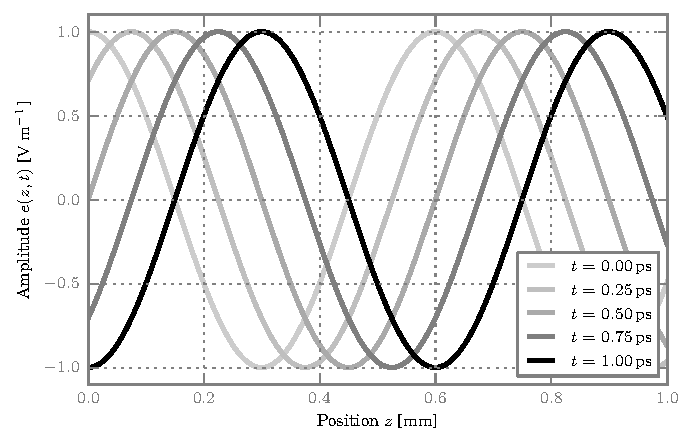
\includegraphics{plane_wave_propagation}
    \caption {\label{fig:plane_wave_propagation}Electric field amplitude of a wave of frequency \SI{500}{\giga\hertz} and amplitude \SI{1}{\volt\per\meter} propagating in vacuum (refractive index 1).}
\end{figure}

In \cref{eq:e_z_t_real}, $t$ is the time coordinate and~$z$ the space coordinate.
$\varphi$ is related to initial conditions and the choice of reference frame.
$E_0$ is the amplitude of the electric field.
It has the dimension of an electric potential per unit length.
It is given for example in volts per meter or newtons per coulomb.

\begin{table}
    \centering
    \caption{Notations and definitions of electromagnetic constants and parameters}
    \caption*{All the entries in this table are real numbers.}
    \label{tab:definitions_simple}
    \rowcolors{2}{gray!25}{white}
    \begin{tabularx}{\textwidth}{l l X}
        \toprule
        \hiderowcolors
        notation & definition & name \\
        \showrowcolors
        \midrule
        $\omega$      &  $2 \pi f$   &  angular frequency \\
        $k$           &  $2 \pi / \lambda$   &   wave number or angular frequency\\
        $\lambda$     &  $c / f$  &  wavelength \\
        $c$           &  $c_0 / n$  &  phase velocity \\
        $c_0$         &  $=\SI{299792458}{\meter\per\second}$  &  speed of light in vacuum \\
        $n$           &  $\sqrt{\epsilon_r \mu_r}$  &  refractive index \\
        $\epsilon_r$  &  $\epsilon / \epsilon_0$  &  relative permittivity or electric constant\\
        $\mu_r$       &  $\mu / \mu_0$  &  relative permeability or magnetic constant\\
        $\epsilon$    & measured material property & absolute permittivity \\
        $\mu$         & measured material property & absolute permeability \\
        $\epsilon_0$  & $\approx \SI{8.854187817e-12}{\farad\per\meter}$  &  absolute permittivity of vacuum \\
        $\mu_0$       & $\approx \SI{1.2566370614e-6}{\henry\per\meter}$  &  absolute permeability of vacuum \\
        $\eta$        & $\sqrt{\mu / \epsilon}$  &  intrinsic impedance \\
        $\eta_0$      & $\sqrt{\mu_0 / \epsilon_0}$  &  intrinsic impedance of free space \\
        $Z$           & $E / H$  & wave impedance \\
        \bottomrule
    \end{tabularx}
\end{table}

\Cref{tab:definitions_simple} summarizes the relations between various parameters used to describe a wave and its propagation medium.
For plane waves in homogeneous materials, $Z=\eta$.
All the parameters introduced in this table are real numbers.
It is possible to add more parameters, such as the electric conductivity of a material.
Such parameters account for attenuation, phase delays, etc.
However, these are more easily dealt with when using complex numbers without changing any of these equations.
In \cref{sec:polar_complex_notation}, we will go over these parameters again and explore the effects of giving them an imaginary part.


%=============================================================================
\subsection{Polar complex notation}
\label{sec:polar_complex_notation}
Euler's formula, given in \cref{eq:euler_formula}, relates the trigonometric function $\cos$ to a complex exponential.
\begin{equation}    
    \exp(i\theta) = \cos(\theta) + i\sin(\theta) \label{eq:euler_formula}
\end{equation}
In \cref{eq:euler_formula}, $i$ represents the imaginary unit such that $i^2=-1$.
If we rewrite the expression of~$E$ given in \cref{eq:e_z_t_real_minus} as a complex in polar coordinates, we have \cref{eq:e_z_t_complex_minus}.
\begin{align}
   \hat{E}(z, t) &= E_0 \exp(i(kz - \omega t + \varphi))
   \label{eq:e_z_t_complex_minus}
   \\
   E(z, t) &= \Re(\hat{E}(z, t))
   \label{eq:e_z_t_real_complex_minus}
\end{align}
The hat above the $E$ signals that $\hat{E}$ is the complex equivalent of $E$.
As shown by \cref{eq:e_z_t_real_complex_minus}, $E$ and $\hat{E}$ do not have the same value (one is real, the other is complex);
however, both describe the same physical phenomenon.

If we open the door to complex numbers, we may want to consider the effect of giving an imaginary part to the parameters of \cref{tab:definitions_simple}.

The imaginary part of the complex angular frequency $\hat{\omega} = \omega' + i \omega''$ corresponds to an amplification of the wave in time, see \cref{eq:complex_angular_frequency}.
If the imaginary part is negative, then the effect is an attenuation of the signal as time goes.
\begin{subequations}
    \begin{align}
       \hat{E}(z, t) &=
       E_0 \exp(i(kz - \hat{\omega} t + \varphi))
       \\
       &=
       E_0 \exp(i(kz - (\omega' + i \omega'') t + \varphi))
       \\
       &=
       E_0 \exp(i(kz - \omega' t + \varphi)) \exp(\omega'' t)
    \end{align}
    \label{eq:complex_angular_frequency}
\end{subequations}
This can be used to model systems that vary in time.
Since the systems we study in this book are time-invariant, $\omega$ will always be real for us.

Folowing the same reasoning, the imaginary part of the complex wavenumber $\hat{k} = k' + i k''$ corresponds to a spatial attenuation or amplification.
See \cref{eq:complex_wavenumber}.
If $k''> 0$, then the wave is attenuated as it propagates.
This can model losses in a material.
\begin{subequations}
    \begin{align}
       \hat{E}(z, t) &=
       E_0 \exp(i(\hat{k}z - \omega t + \varphi))
       \\
       &=
       E_0 \exp(i((k' + i k'')z - \omega t + \varphi))
       \\
       &=
       E_0 \exp(i(k' z - \omega t + \varphi)) \exp(-k'' z)
    \end{align}
    \label{eq:complex_wavenumber}
\end{subequations}
Having $k'' \ne 0$ gives an imaginary part to the wavelength and the phase velocity
(see \cref{tab:definitions_simple}).
All these imaginary parts mean the same thing: the wave is getting attenuated.
However, the speed of light in vacuum is known to be a real number.
Therefore, the imaginary part of $\hat{k}$ comes from an imaginary part of the complex refractive index $\hat{n}$.
This links the attenuation of the wave to a property of the material.
Since the refractive index is derived from the relative electric permittivity and the relative magnetic permeability of a materials
($\hat{n}=\sqrt{\hat{\epsilon}\hat{\mu}}$),
any of them can be responsible for the attenuation of the wave.

When using Snell's law \eqref{eq:snell}, the real part of the refractive indices must be used.

In many cases (vacuum, mylar, aluminum), the relative magnetic permeability is very close to 1, making the electric permitivity the only parameter able to bear an imaginary part.
This means that, in these cases, the wave is absorbed by a material because of its conductivity.
The conductivity $\sigma$ and the imaginary part of the permittivity $\epsilon''$ are bound by \cref{eq:epsilon_second_sigma}.
The higher the frequency, the less effect the conductivity has.
This is understandable as inertia prevents the electrons from moving fast enough to cancel the electric field.
\begin{equation}   
    \epsilon'' = \sigma / \omega
    \label{eq:epsilon_second_sigma}
\end{equation}
The conductivity itself can be complex, in which case its imaginary part acts like a frequency-dependant real part of the permittivity.

In some cases, the relative magnetic permeability is very different from~1 and is able to go up to several thousands in the case of very pure iron.
It can a priori be complex.
\citeauthor{bowler2006frequency} has shown in \citetitle{bowler2006frequency} \cite{bowler2006frequency} that the imaginary part of the permeability is frequency dependant.
However, that frequency dependance of $\mu''$ does not seem as simple as that of $\epsilon''$.

Finally, the complex intrinsic impedance derived from the complex permittivity and permeability imply that the electric and magnetic fields are not in phase.
Indeed, for a plane wave in a homogeneous material, the wave impedance $\hat{Z}=\hat{E}/\hat{H}$ equals the intrinsic impedance $\hat{\eta}=\sqrt{\hat{\mu}/\hat{\epsilon}}$.
Therefore, the imaginary part of $\hat{\mu}$ or $\hat{\epsilon}$ creates a phase difference between $\hat{E}$ and $\hat{H}$.

%=============================================================================
\subsection{Phasors}
\index{phasor}

\subsubsection{Introducing phasors}
By applying the exponentiation identity \cref{eq:exponentiation_identity},
\cref{eq:e_z_t_complex_minus} can also be written as \cref{eq:e_z_t_complex_factorized}.
\begin{equation}
    \exp(a+b) = \exp(a) \exp(b)
    \label{eq:exponentiation_identity}
\end{equation}
\begin{equation}
    \hat{E}(z, t)
    =
    E_0 \exp(ikz) \exp(-i\omega t) \exp({i \varphi})
    \label{eq:e_z_t_complex_factorized}
\end{equation}
In \cref{eq:e_z_t_complex_factorized}, the expression of the wave is separated into four independant factors.
This is possible because the amplitude $E_0$, the wavenumber $k$, the angular frequency $\omega$ and the phase $\varphi$ are time-invariant.
The time-invariance of $\omega$ and $k$ is guaranteed by the linearity hypothesis, while that of $E_0$ and $\varphi$ is guaranteed by the coherency hypothesis.

The time factor $\exp({-i \omega t})$ is common to all the waves present in the system.
Because of that, we can factor it out as shown in equations~\ref{eq:factor_time_out} and \ref{eq:phasor}.
In these equations, $\hat{E}(z)$ is a ``phasor representation'' of the sinusoidal function $E(z, t)$, with the time factored out and considered implicit.
\begin{align}
    \hat{E}(z, t) &= \hat{E}(z) \exp(-i\omega t) \label{eq:factor_time_out}
    \\
    \hat{E}(z) &= E_0 \exp(i(kz+\varphi)) \label{eq:phasor}
\end{align}

The term ``phasor'' is a portmanteau of ``phase vector'', indicating that $\hat{E}(z)$ can be visualized as a vector on the complex plane, and that $\hat{E}(z, t)$ makes that vector rotate with time.

\subsubsection{Convention}
We have shown with equations~\ref{eq:e_z_t_real_minus} and \ref{eq:e_z_t_real_plus} that there are two conventions for representing the same physical phenomenon.
Either the space factor or the time factor takes a negative sign, and that decision is a priori arbitrary.

The choice of convention influences the definition of our phasors.
We have to choose between
\cref{eq:phasor_minus} and \cref{eq:phasor_plus}.
\begin{subequations}
    \begin{align}
        \text{Either }
        \hat{E}(z) &= E_0 \exp(i(kz+\varphi))
        \label{eq:phasor_minus}
        \\
        \text{or }
        \hat{E}(z) &= E_0 \exp(i(-kz-\varphi))
        \text{.}
         \label{eq:phasor_plus}
    \end{align}    
\end{subequations}

For simplicity, we choose \cref{eq:phasor_minus}.
Indeed, it does not carry a negative sign.
The negative sign is factored out in the time-factor $\exp{-i \omega t}$.


\subsubsection{Discrete space}
In our optical systems, we are hardly ever interested in the value of the phasor at any point.
For example, when modeling the effect of a dielectric interface on a wave, we need only to know the value of the phasor at the location of the interface.
If there are two interfaces, then there are two points of interest.
This means that we do not keep the explicit dependency on $z$ in our computations but work with discrete values of $z$ as illustrated by \cref{eq:phasor_no_z}.
\begin{equation}
    \begin{aligned}
        \hat{E}_0 &= E_0 \exp(i(k_0 z_0 + \varphi_0))
        \\
        \hat{E}_1 &= E_1 \exp(i(k_1 z_1 + \varphi_1))
    \end{aligned}
    \label{eq:phasor_no_z}
\end{equation}
In \cref{eq:phasor_no_z}, the phasors $\hat{E}_n$ do not depend on a space coordinate because they are defined for a specific location.
This is the type of phasors that we will be using in the rest of our chapter.

\subsubsection{Phasor algebra}
Phasors can be added together to produce a new phasor.
Physically, this corresponds to adding together the electric fields of different waves.
This is by adding phasors that we model interferences.

A phasor can be multiplied by a scalar to produce a new phasor.
The scalar can be a complex number, but that does not make this scalar a phasor. 
The real part of the scalar models the gain or absorption, while the imaginary part models the phase shift.
The scalar multiplication models the effect of an optical element on a wave.

Phasors cannot be multiplied together.
In algebraic terms, phasors form a vector space, not a ring.
The product of two phasors would represent the product of two sinusoids which is a non-linear operation that introduce new frequencies.
Since phasors can represent systems with one frequency only, the result of multiplying two phasors is not a phasor.
This means that computing the power transported by a wave is more subtle than just squaring the phasor, which we will study in \vref{sec:jones_vectors_and_power}.


%=============================================================================
\subsection{Scattering matrices}
Scattering matrices \cite{siegman1986lasers} model the transfer of power or field from one side (port) of a network to another (\cref{fig:scattering_matrix_notations}).
In coherent systems, they operate on phasors and therefore manipulate the field, not the power.

\Cref{eq:scattering_matrix} presents the scattering matrix $S$ that models the relation between a vector of inputs $a$ and a vector of outputs $b$ for a $n$-ports network.
The diagonal contains the reflections terms and the rest contains the transmissions.
\begin{align}
    b &= S a
    &
    \begin{pmatrix}
        b_1\\
        b_2\\
        \vdots\\
        b_n
    \end{pmatrix}
    &=
    \begin{pmatrix}
        S_{1, 1} & S_{1, 2} & \cdots & S_{1, n} \\
        S_{2, 1} & S_{2, 2} & \cdots & S_{2, n} \\
        \vdots   & \vdots   & \ddots & \vdots   \\
        S_{n, 1} & S_{n, 2} & \cdots & S_{n, n}
    \end{pmatrix}
    \begin{pmatrix}
        a_1\\
        a_2\\
        \vdots\\
        a_n
    \end{pmatrix}
    \label{eq:scattering_matrix}
\end{align}

\begin{figure}[hbtp]
    \centering
    \input{scattering_matrix_notations.pdf_tex}
    \caption{A 4-ports network showing 4 inputs $a_i$ and four outputs $b_i$.  For example, this network could be a wire grid polarizer or a semi-transparent mirror, both acting as beam splitters.}%
    \label{fig:scattering_matrix_notations}
\end{figure}

In the general case, scattering matrices cannot be multiplied together.
The scattering matrix of a system of two networks is not the product of the scattering matrices of the individual networks.
We will explore this further in \cref{sec:solving_a_system}.

Scattering matrices are firstly designed to model discrete physical optical elements such as interfaces, distances, horns, grids, etc.
It is possible to extend their use to an entire system made of several networks as long as it provides outputs that are linear combinations of inputs.
We will also explore this further in \cref{sec:solving_a_system}.



%=============================================================================
\subsection{Jones calculus in 3D}

%-----------------------------------------------------------------------------
\subsubsection{Traditional Jones calculus}
Jones matrices model the transfer of amplitude and phase from one polarization to another \cite{hecht2002optics}.
In \cref{eq:jones_matrix_short}, the polarized input field $\vect{\hat{E}}_i$ is related to the polarized output field~$\vect{\hat{E}}_o$ by the Jones matrix $J$.
$\vect{\hat{E}}_i$ and $\vect{\hat{E}}_o$ are called ``Jones vectors''.
\begin{equation}
    % Small form.
    \vect{\hat{E}}_o = J \vect{\hat{E}}_i
    \label{eq:jones_matrix_short}
\end{equation}
The components of the Jones vectors are phasors: complex numbers that encode the amplitude and phase of the field along different axes.
The components of the Jones matrices are als numbers, these encode changes in amplitude and phase.

\Cref{eq:jones_matrix_2d} presents the traditional form of Jones vectors and matrices.
\begin{equation}
    % Jones matrix in 2D.
    \begin{pmatrix}
        \hat{E}_{o, h}\\
        \hat{E}_{o, v}
    \end{pmatrix}
    =
    \begin{pmatrix}
        J_{h, h}   &   J_{h, v} \\
        J_{v, h}   &   J_{v, v}
    \end{pmatrix}
    \begin{pmatrix}
        \hat{E}_{i, h}\\
        \hat{E}_{i, v}
    \end{pmatrix}
    \label{eq:jones_matrix_2d}
\end{equation}
The field is seen as the superposition of a horizontal and a vertical component, both linearly polarized.
The phase difference between these components determines the handedness and the ellipticity of the polarization of the field.

%-----------------------------------------------------------------------------
\subsubsection{Extension to three dimensions}
Although very useful for many applications, the traditional Jones matrices and vectors have limitations.
First, the field is always expressed in a local reference frame: the horizontal and vertical directions are valid for one beam only and may change after any reflection or refraction.
Therefore, to completely describe a field, the Jones vector is not enough since one needs to keep track of the orientation of its reference frame with three angles, a quaternion or a rotation matrix.

Second, the horizontal and vertical directions are normal to each other and to the direction of propagation.
This limits us to modeling either transverse electric or transverse magnetic waves depending on whether the Jones vector represents the electric or the magnetic field;
this cannot model hybrid waves, in which both the electric and the magnetic field can have a component along the direction of propagation.
Therefore, this cannot model propagation in a birefringent material.
One way to accommodate this is to relax the constraint of orthogonality of the reference frame, allowing for the horizontal and vertical directions to have a component along the direction of propagation.
If we do this, then the full description of the field gets even more complicated as we need to carry along, not just the orientation of its reference frame, but the full description of that non-Cartesian reference frame.

Instead, we can express all the fields in a common global Cartesian reference frame, essentially extending Jones calculus from two to three dimensions, as illustrated in \cref{eq:jones_matrix_3d}.
\begin{equation}
    % Jones matrix in 3D.
    \begin{pmatrix}
        \hat{E}_{o, x}\\
        \hat{E}_{o, y}\\
        \hat{E}_{o, z}
    \end{pmatrix}
    =
    \begin{pmatrix}
        J_{x, x}   &   J_{x, y}   &   J_{x, z} \\
        J_{y, x}   &   J_{y, y}   &   J_{y, z} \\
        J_{z, x}   &   J_{z, y}   &   J_{z, z}
    \end{pmatrix}
    \begin{pmatrix}
        \hat{E}_{i, x}\\
        \hat{E}_{i, y}\\
        \hat{E}_{i, z}
    \end{pmatrix}
    \label{eq:jones_matrix_3d}
\end{equation}
These Jones matrices can be combined with rotation matrices (built from Euler angles or quaternions) in order to represent networks in any orientation in space.

%-----------------------------------------------------------------------------
\subsubsection{Rotating Jones matrices}
\label{sec:rotating_jones_matrices}
If $R$ is a 3--by--3 rotation matrix and $J$ the Jones matrix of a network at rest,
then \cref{eq:jones_rotation_using_inverse} gives the Jones matrix $J'$ corresponding to that network rotated by $R$.

\begin{equation}
    J' = R J R^{-1}
    \label{eq:jones_rotation_using_inverse}
\end{equation}
\Cref{eq:jones_rotation_using_inverse} is correct, however it may not be the most practical to implement.
Indeed, inverting matrices is an expensive and unstable operation for a computer to perform
When we remember that the inverse of a rotation matrix is also its transpose%
\todo{citation needed},
then we get \cref{eq:jones_rotation_using_transpose} which has the advantage of being computationally cheap and stable.
\begin{equation}
    J' = R J R\transp
    \label{eq:jones_rotation_using_transpose}
\end{equation}

Rotating the identity matrix has an interesting property shown by~\eqref{eq:jones_rotation_identity}.
\begin{equation}
    I' = R I R^{-1}
       = R R^{-1}
       = I
    \label{eq:jones_rotation_identity}
\end{equation}
If a Jones matrix is proportional to an identity matrix, then it is not modified by rotation.
We will use that property to save some computation, for example when propagating through homogeneous isotropic materials (\vref{sec:generic_networks_distance}).



%=============================================================================
\subsection{Jones vectors and power}
\label{sec:jones_vectors_and_power}
When dealing with complex numbers, we must carefully define what we mean by ``power''.
\citetitle{IEEE2002dictionary} \cite{IEEE2002dictionary} defines the following terms and SI units:
\begin{description}
    \item[complex power]\quad%
    $\hat{S} = P + iQ$\quad%
    in \si{\volt\ampere} (volt-ampere),
    \item[active/real power]\quad%
    $P \in \mathbb{R} = \Re(\hat{S})$\quad%
    in \si{\watt} (watt),
    \item[reactive power]\quad%
    $Q \in \mathbb{R} = \Im(\hat{S})$\quad%
    in \si{var} (volt-ampere-reactive),
    \item[apparent power]\quad%
    $\abs{\hat{S}} = \sqrt{P^2 + Q^2}$\quad%
    in \si{\volt\ampere} (volt-ampere).
\end{description}
In our case, we deal with power densities: instead of watt, we use watt per square meter.
We can define ``complex power density'', ``active power density'', ``reactive power density'' and ``apparent power density'' by taking the correspondant absolute powers from the list above and normalizing them by a unit surface area.
For simplicity, we keep the same notations.

Considering that the electric field is given in volt per meter and the magnetic field in ampere per meter, their product yields a quantity that has the dimension of a power density.
It is tempting to write $\hat{S}=\hat{E}\hat{H}$ with $\hat{E}$ and $\hat{H}$ phasors;
however this is incorrect for two reasons:
\begin{enumerate}
    \item each phasor represents a sinusoidal signal, and the product of two sinusoids is a non-linear operation that introduces new frequencies,
    \item our electric and magnetic fields are three dimensional, they are Jones vectors.
\end{enumerate}

\index{Poynting vector}The ``Poynting vector'' represents the directional energy flux density of an electromagnetic wave, typically expressed in \si{\watt\per\meter\squared}.
Traditionally noted~$\vect{S}$, it is defined by \cref{eq:poynting_vector}.
This vector takes care of the fact that the electric and magnetic fields ($\vect{E}$ and $\vect{H}$) are three dimensional vectors.
However, as indicated by the absence of hat symbols, the components of $\vect{E}$, $\vect{H}$ and $\vect{S}$ are real numbers, not complex numbers.
This means that we cannot use phasors directly in this equation.
The letter~$\vect{S}$ here must not be confused with the~$\hat{S}$ above which corresponds to a complex power.
Actually, since the Poynting vector deals with real values, it has more affinities with the active power density $P$.
\begin{equation}
    \vect{S} = \vect{E} \times \vect{H} \label{eq:poynting_vector}
\end{equation}
The definition of this Poynting vector holds even for anisotropic propagation media for which $\vect{E}$, $\vect{H}$ and the wave vector $\vect{k}$ may not be normal to each other.
Since the Poynting vector is defined by a cross product, it is by definition normal to the electric and magnetic field, even if that direction differs from $\vect{k}$.

Since the active power is a priori the most interesting (sources emit real power, and detectors detect real power), let us compute the Poynting vector from $\vect{\hat{E}}$ and $\vect{\hat{H}}$, both three dimentional vectors with phasors components.

In order to avoid non-linearities, the first thing to do is to express the electric and magnetic field with their time factor.
This is shown in \cref{eq:e_h_time}, where the components of $\vect{\hat{E}}(t)$ and $\vect{\hat{H}}(t)$ are not phasors anymore but complex amplitudes.
They are no more representations of sinusoidal functions, they are specific values of these functions.
\begin{subequations}
    \begin{align}
        \vect{\hat{E}}(t) = \vect{\hat{E}} \exp(-i \omega t) \\
        \vect{\hat{H}}(t) = \vect{\hat{H}} \exp(-i \omega t)
    \end{align}
    \label{eq:e_h_time}
\end{subequations}

The second step is to take their real values.
This is what we do with \crefrange{eq:e_time_real_0}{eq:e_time_real_2} for the electric field.
The same equations can be applied to the magnetic field.
These equations are applied on the three components of the vectors independently.
\begin{subequations}
\begin{align}
    \vect{E}(t) &= \Re
    \bigg(
        \Big(
            \Re(\vect{\hat{E}}) + i \Im(\vect{\hat{E}})
        \Big)
        \Big(
            \cos(- \omega t) + i \sin(- \omega t)
        \Big)
    \bigg)
    \label{eq:e_time_real_0}
    \\
    \vect{E}(t) &= \Re(\vect{\hat{E}}) \cos(- \omega t)
            -
            \Im(\vect{\hat{E}}) \sin(- \omega t)
    \label{eq:e_time_real_1}
    \\
    \vect{E}(t) &= \Re(\vect{\hat{E}}) \cos(\omega t)
            +
            \Im(\vect{\hat{E}}) \sin(\omega t)
    \label{eq:e_time_real_2}
\end{align}
    \label{eq:e_time_real}
\end{subequations}

The third step is to compute the cross product of $\vect{E}(t)$ and $\vect{H}(t)$ to get the Poynting vector $\vect{S}(t)$.
For brevity, let us pose $c=\cos(\omega t)$, $s=\sin(\omega t)$,
$\vect{E}_r = \Re(\vect{\hat{E}})$, $\vect{E}_i = \Im(\vect{\hat{E}})$,
$\vect{H}_r = \Re(\vect{\hat{H}})$ and $\vect{H}_i = \Im(\vect{\hat{H}})$.
The Poynting vector is then given by \cref{eq:e_cross_h}.
\begin{equation}
    \vect{S}(t)
    =
    \begin{pmatrix}
         (E_{iy} s + E_{ry} c) (H_{iz} s + H_{rz} c) -
         (E_{iz} s + E_{rz} c) (H_{iy} s + H_{ry} c)
         \\
         (E_{iz} s + E_{rz} c) (H_{ix} s + H_{rx} c) -
         (E_{ix} s + E_{rx} c) (H_{iz} s + H_{rz} c)
         \\
         (E_{ix} s + E_{rx} c) (H_{iy} s + H_{ry} c) -
         (E_{iy} s + E_{ry} c) (H_{ix} s + H_{rx} c)
    \end{pmatrix}
    \label{eq:e_cross_h}
\end{equation}
Expanding the components yields many $\cos(\omega t)^2$, $\sin(\omega t)^2$ and $\cos(\omega t)\sin(\omega t)$.

The Poynting vector is a instantaneous quantity; it is defined for a specific instant $t$.
It is possible to define a time-averaged Poynting vector $\vect{\bar{S}}$ with \cref{eq:pointing_average}.
\begin{equation}
    \vect{\bar{S}} = \frac{1}{T}
    \int_0^T \! \vect{S}(t)\, \mathrm{d}t
    \label{eq:pointing_average}
\end{equation}
In \cref{eq:pointing_average}, $T$ is the period of the signal defined by $T=1/f$ and $f=\omega/2\pi$.
The time-average of the $\sin^2$, $\cos^2$ and $\sin\cos$ functions found in the Poynting vectors are given by \crefrange{eq:trig_average_ss}{eq:trig_average_sc}.
\begin{subequations}
    \begin{align}
        \frac{1}{T} &\int_0^{T} \! \sin(\omega t)^2 \, \mathrm{d}t = \frac{1}{2}
        \label{eq:trig_average_ss}
        \\
        \frac{1}{T} &\int_0^{T} \! \cos(\omega t)^2 \, \mathrm{d}t = \frac{1}{2}
        \label{eq:trig_average_cc}
        \\
        \frac{1}{T} &\int_0^{T} \! \sin(\omega t)\cos(\omega t) \, \mathrm{d}t = 0
        \label{eq:trig_average_sc}
    \end{align}
    \label{eq:trig_average}
\end{subequations}
Using this, the time-averaged Poynting vector $\vect{\bar{S}}$ is easy to derive from \cref{eq:e_cross_h}.
\Crefrange{eq:poynting_average_detail_0}{eq:poynting_average_detail_3} detail that process.
\begin{subequations}
\begin{align}
    \vect{\bar{S}}
    &= \frac{1}{2}
    \begin{pmatrix}
        (E_{iy}H_{iz} + E_{ry}H_{rz}) -
        (E_{iz}H_{iy} + E_{rz}H_{ry})
        \\
        (E_{iz}H_{ix} + E_{rz}H_{rx}) -
        (E_{ix}H_{iz} + E_{rx}H_{rz})
        \\
        (E_{ix}H_{iy} + E_{rx}H_{ry}) -
        (E_{iy}H_{ix} + E_{ry}H_{rx})
    \end{pmatrix}
    \label{eq:poynting_average_detail_0}
    \\
    &= \frac{1}{2}
    \begin{pmatrix}
        (E_{iy}H_{iz} - E_{iz}H_{iy}) + 
        (E_{ry}H_{rz} - E_{rz}H_{ry})
        \\
        (E_{iz}H_{ix} - E_{ix}H_{iz}) + 
        (E_{rz}H_{rx} - E_{rx}H_{rz})
        \\
        (E_{ix}H_{iy} - E_{iy}H_{ix}) +
        (E_{rx}H_{ry} - E_{ry}H_{rx})
    \end{pmatrix}
    \label{eq:poynting_average_detail_1}
    \\
    &= \frac{1}{2}
    \left[
    \begin{pmatrix}
        E_{iy}H_{iz} - E_{iz}H_{iy} \\
        E_{iz}H_{ix} - E_{ix}H_{iz} \\
        E_{ix}H_{iy} - E_{iy}H_{ix} 
    \end{pmatrix}
    +
    \begin{pmatrix}
        E_{ry}H_{rz} - E_{rz}H_{ry} \\
        E_{rz}H_{rx} - E_{rx}H_{rz} \\
        E_{rx}H_{ry} - E_{ry}H_{rx}        
    \end{pmatrix}
    \right]
    \label{eq:poynting_average_detail_2}
    \\
    &= \frac{1}{2}
    \left[
        \vect{E}_i \times \vect{H}_i
    +
        \vect{E}_r \times \vect{H}_r
    \right]
    \label{eq:poynting_average_detail_3}
\end{align}
\end{subequations}
We remember that $\vect{E}_i$ is a short hand notation for the imaginary part of the electric Jones vector $\vect{\hat{E}}$, etc.
This means that the time-averaged Poynting vector $\vect{\bar{S}}$ can be calculated directly from the Jones vectors $\vect{\hat{E}}$ and $\vect{\hat{H}}$, as shown in \cref{eq:poynting_from_phasors}.
\begin{equation}
    \vect{\bar{S}} = \frac{1}{2}
    \left(
        \Re(\vect{\hat{E}}) \times \Re(\vect{\hat{H}}) + 
        \Im(\vect{\hat{E}}) \times \Im(\vect{\hat{H}})
    \right)
    \label{eq:poynting_from_phasors}
\end{equation}
\Cref{eq:poynting_from_phasors} gives the real averaged power density of a wave described by its electric and magnetic Jones vectors.
If $\vect{\hat{H}}$ is unknown, it can be retreived from the electric field with a variant of Ohm's law \eqref{eq:ohm_law} using the wave impedance matrix $\hat{Z}$.
In homogeneous isotropic materials, the impedance matrix equals the scalar impedance multiplied by the matrix of a $+\pi/2$ rotation around~$\vect{k}$.
\begin{equation}
    \vect{\hat{E}} = \hat{Z} \vect{\hat{H}} \label{eq:ohm_law}
\end{equation}
This is how we compute the power of a wave described by its Jones vector~$\vect{\hat{E}}$.



%=============================================================================
\subsection{Combining scattering and Jones matrices}
We repeat here the definition of a scattering matrix given by \vref{eq:scattering_matrix}.
\begin{align*}
    b &= S a
    &
    \begin{pmatrix}
        b_1\\
        b_2\\
        \vdots\\
        b_n
    \end{pmatrix}
    &=
    \begin{pmatrix}
        S_{1, 1} & S_{1, 2} & \cdots & S_{1, n} \\
        S_{2, 1} & S_{2, 2} & \cdots & S_{2, n} \\
        \vdots   & \vdots   & \ddots & \vdots   \\
        S_{n, 1} & S_{n, 2} & \cdots & S_{n, n}
    \end{pmatrix}
    \begin{pmatrix}
        a_1\\
        a_2\\
        \vdots\\
        a_n
    \end{pmatrix}
\end{align*}

Each port of an optical network receives and emits a polarized wave.
Since Jones vectors describe polarized waves, it is natural to model each input and output with a Jones vector.
This makes $a$ and $b$ vectors of Jones vectors.
As a consequence, each element $S_{i, j}$ of the scattering matrix S is a Jones matrix.
We are dealing with vectors of vectors and matrices of matrices, as shown by \cref{eq:matrix_of_matrices} for a 2-ports network.

\begin{equation}
    \begin{gathered}
    \begin{pmatrix}
        \begin{pmatrix}
            \hat{b}_{1, x} \\ \hat{b}_{1, y} \\ \hat{b}_{1, z}
        \end{pmatrix}
        \\
        \begin{pmatrix}
            \hat{b}_{2, x} \\ \hat{b}_{2, y} \\ \hat{b}_{2, z}
        \end{pmatrix}
    \end{pmatrix}
    =
    S
    \begin{pmatrix}
        \begin{pmatrix}
            \hat{a}_{1, x} \\ \hat{a}_{1, y} \\ \hat{a}_{1, z}
        \end{pmatrix}
        \\
        \begin{pmatrix}
            \hat{a}_{2, x} \\ \hat{a}_{2, y} \\ \hat{a}_{2, z}
        \end{pmatrix}
    \end{pmatrix}
    \\
    S =
    \begin{pmatrix}
        \begin{pmatrix}
            S_{1, 1, x, x} & S_{1, 1, x, y} & S_{1, 1, x, z} \\
            S_{1, 1, y, x} & S_{1, 1, y, y} & S_{1, 1, y, z} \\
            S_{1, 1, z, x} & S_{1, 1, z, y} & S_{1, 1, z, z} \\
        \end{pmatrix}
        &
        \begin{pmatrix}
            S_{1, 2, x, x} & S_{1, 2, x, y} & S_{1, 2, x, z} \\
            S_{1, 2, y, x} & S_{1, 2, y, y} & S_{1, 2, y, z} \\
            S_{1, 2, z, x} & S_{1, 2, z, y} & S_{1, 2, z, z} \\
        \end{pmatrix}
        \\
        \begin{pmatrix}
            S_{2, 1, x, x} & S_{2, 1, x, y} & S_{2, 1, x, z} \\
            S_{2, 1, y, x} & S_{2, 1, y, y} & S_{2, 1, y, z} \\
            S_{2, 1, z, x} & S_{2, 1, z, y} & S_{2, 1, z, z} \\
        \end{pmatrix}
        &
        \begin{pmatrix}
            S_{2, 2, x, x} & S_{2, 2, x, y} & S_{2, 2, x, z} \\
            S_{2, 2, y, x} & S_{2, 2, y, y} & S_{2, 2, y, z} \\
            S_{2, 2, z, x} & S_{2, 2, z, y} & S_{2, 2, z, z} \\
        \end{pmatrix}
    \end{pmatrix}
    \end{gathered}
    \label{eq:matrix_of_matrices}
\end{equation}

Although matrices of matrices are compabible with simple algebraic operations (the product above follows the usual rule for multiplying matrices), we prefer to interpret them as more conventional ``block matrices''.
Block matrices are described by \citeauthor{eves2012elementary} in \citetitle{eves2012elementary} \cite{eves2012elementary}.
They are conventional matrices, in the sense that they hold scalars, but they are subdivided in regions, or ``blocks''.
Mathematically, \cref{eq:matrix_of_matrices} is equivalent to \cref{eq:matrix_flattenned}.
\begin{equation}
    \begin{pmatrix}
        \hat{b}_{1, x} \\ \hat{b}_{1, y} \\ \hat{b}_{1, z}
        \\
        \hat{b}_{2, x} \\ \hat{b}_{2, y} \\ \hat{b}_{2, z}
    \end{pmatrix}
    =
    \begin{pmatrix}
        S_{1, 1, x, x} & S_{1, 1, x, y} & S_{1, 1, x, z}   &   S_{1, 2, x, x} & S_{1, 2, x, y} & S_{1, 2, x, z} \\
        S_{1, 1, y, x} & S_{1, 1, y, y} & S_{1, 1, y, z}   &   S_{1, 2, y, x} & S_{1, 2, y, y} & S_{1, 2, y, z} \\
        S_{1, 1, z, x} & S_{1, 1, z, y} & S_{1, 1, z, z}   &   S_{1, 2, z, x} & S_{1, 2, z, y} & S_{1, 2, z, z} \\
        S_{2, 1, x, x} & S_{2, 1, x, y} & S_{2, 1, x, z}   &   S_{2, 2, x, x} & S_{2, 2, x, y} & S_{2, 2, x, z} \\
        S_{2, 1, y, x} & S_{2, 1, y, y} & S_{2, 1, y, z}   &   S_{2, 2, y, x} & S_{2, 2, y, y} & S_{2, 2, y, z} \\
        S_{2, 1, z, x} & S_{2, 1, z, y} & S_{2, 1, z, z}   &   S_{2, 2, z, x} & S_{2, 2, z, y} & S_{2, 2, z, z}
    \end{pmatrix}
    \begin{pmatrix}
        \hat{a}_{1, x} \\ \hat{a}_{1, y} \\ \hat{a}_{1, z}
        \\
        \hat{a}_{2, x} \\ \hat{a}_{2, y} \\ \hat{a}_{2, z}
    \end{pmatrix}
    \label{eq:matrix_flattenned}
\end{equation}

This equivalence means that we can see each polarization of each port as a full-fledged port, and that the same physical phenomenon could be modeled with a 6-ports network described by \cref{eq:matrix_totally_flattenned}.
\begin{equation}
    \begin{pmatrix}
        \hat{b}'_1 \\ \hat{b}'_2 \\ \hat{b}'_3 \\ \hat{b}'_{4} \\ \hat{b}'_{5} \\ \hat{b}'_{6}
    \end{pmatrix}
    =
    \begin{pmatrix}
        S'_{1, 1} & S'_{1, 2} & S'_{1, 3} & S'_{1, 4} & S'_{1, 5} & S'_{1, 6} \\
        S'_{2, 1} & S'_{2, 2} & S'_{2, 3} & S'_{2, 4} & S'_{2, 5} & S'_{2, 6} \\
        S'_{3, 1} & S'_{3, 2} & S'_{3, 3} & S'_{3, 4} & S'_{3, 5} & S'_{3, 6} \\
        S'_{4, 1} & S'_{4, 2} & S'_{4, 3} & S'_{4, 4} & S'_{4, 5} & S'_{4, 6} \\
        S'_{5, 1} & S'_{5, 2} & S'_{5, 3} & S'_{5, 4} & S'_{5, 5} & S'_{5, 6} \\
        S'_{6, 1} & S'_{6, 2} & S'_{6, 3} & S'_{6, 4} & S'_{6, 5} & S'_{6, 6}
    \end{pmatrix}
    \begin{pmatrix}
        \hat{a}'_1 \\ \hat{a}'_2 \\ \hat{a}'_3 \\ \hat{a}'_{4} \\ \hat{a}'_{5} \\ \hat{a}'_{6}
    \end{pmatrix}
    \label{eq:matrix_totally_flattenned}
\end{equation}
Although the term is not canon, we call non-block matrices ``flat'' matrices.
They are flat in the sense that they are two dimensional, while our block matrices have four indices and are therefore four-dimensional.
In this book, we will switch between block matrices and flat matrices at our convenience.




%=============================================================================
\subsection{Solving a system}
\label{sec:solving_a_system}



%-----------------------------------------------------------------------------
\subsubsection{Theory}

We call $S$ the flat scattering matrix of the entire system.
\begin{equation*}
    S =
    \begin{pmatrix}
        S_{1, 1} & S_{1, 2} & \cdots & S_{1, n} \\
        S_{2, 1} & S_{2, 2} & \cdots & S_{2, n} \\
        \vdots   & \vdots   & \ddots & \vdots \\
        S_{n, 1} & S_{n, 2} & \cdots & S_{n, n}
    \end{pmatrix}
\end{equation*}
\begin{equation*}
    b = Sa
\end{equation*}
$S$ contains information about all the ports in the system: the ports that are open to the outside world, but also the ports hidden within the system because the networks are coupled to each other.
Here, $n$ is the number of ports of $S$, equal to the sum of the number of ports of all the networks constituting the system.

Some of the networks constituting the system are coupled by one port.
If two networks G and H are coupled by their port $g$ and $h$, then the output phasor of $g$ is the input phasor of $h$ and the output phasor of $h$ is the input phasor of $g$, as illustrated by \cref{eq:coupled_inputs_outputs}.
\begin{equation}
    \left\lbrace
    \begin{aligned}
        \hat{b}_h &= \hat{a}_g \\
        \hat{b}_g &= \hat{a}_h
    \end{aligned}
    \right.
    \label{eq:coupled_inputs_outputs}
\end{equation}

In the rest of this section, the components of vectors and matrices are are implicitely complex.
In order to lighten the notations, we will not place the hat symbol which we usually use for complex numbers.

Ports that are coupled are called ``inside port'', those that are not coupled are called ``outside port''.
If we note~$a^o$ the inputs from the outside world,~$b^o$ the outputs to the outside world,~$a^i$ the inputs inside the system and~$b^i$ the outputs inside the system, then we can reorder the rows and columns of the vectors~$a$,~$b$ and the matrix~$S$ to put together the inside ports and the outside ports.
This is illustrated by \cref{eq:s_outside_inside} with block matrices separating the inside and outside ports.
\begin{equation}
    \binom{b^o}{b^i} =
    \begin{pmatrix}
        S^{oo} & S^{oi} \\
        S^{io} & S^{ii} \\
    \end{pmatrix}
    \binom{a^o}{a^i}
    \label{eq:s_outside_inside}
\end{equation}
The four regions of~$S$ have the following physical meaning:
\begin{description}
    \item[$S^{oo}$:] from outside to outside: signal that is reflected on the entrance ports and therefore never enters the system.
    \item[$S^{io}$:] from outside to inside: signal that enters the system.
    \item[$S^{ii}$:] from inside to inside: transmissions and reflections internal to the system.
    \item[$S^{oi}$:] from inside to outside: signal that leaves the system.
\end{description}
Of $a$ and $b$, only~$a^o$ is known: this corresponds to the input to the system and we control it.
$a^i$,~$b^i$ and~$b^o$ are unknown.
$b^o$ is the result we are looking for.
$b^i$ and~$a^i$ are nice to have as they allow us to see what is happening inside the system.

\paragraph{Solving the internal transmissions and reflections.}
How are~$a^i$ and~$b^i$ related?
\Cref{eq:coupled_inputs_outputs} indicates that each element of $a^i$ is equal to an element of $b^i$, therefore $a^i$ can be obtain by reordering $b^i$ and vice-versa.
\index{permutation matrix}In other words, there exists a permutation matrix~$P$ such that
\begin{equation}
    a^i = P b^i \text{.} \label{eq:relation_ai_bi}
\end{equation}

To get $b^o$, the first step is to compute~$b^i$ from~$a^o$.
\begin{subequations}
    \begin{align}
        b^i &= S^{io}a^o + S^{ii}a^i \label{eq:compute_bi_ai} \\
        b^i &= S^{io}a^o + S^{ii}Pb^i \label{eq:compute_bi_bi} \\
        (I - S^{ii}P)b^i &= S^{io}a^o \label{eq:compute_bi_solve} \\
        b^i &= (I - S^{ii}P)^{-1} S^{io}a^o \label{eq:compute_bi_invert}
    \end{align} \label{eq:compute_bi}
\end{subequations}
where~$I$ is the identity matrix with a dimension equal to that of~$S^{ii}P$.

Can we go from \cref{eq:compute_bi_solve} to \cref{eq:compute_bi_invert}?
The matrix~$I - S^{ii}P$ has an inverse if and only if it is not singular.
A matrix is singular if and only if its determinant equals~0.
Can the determinant of~$I - S^{ii}P$ equal~0 (\cref{eq:det_i_minus_siip})?
\begin{equation}
    \det(I - S^{ii}P) = 0 \label{eq:det_i_minus_siip}
\end{equation}
\index{eigenvalue}\Cref{eq:det_i_minus_siip} has the shape of an eigenvalue problem;
\cref{eq:eigenvalue_typical} defines the eigenvalues~$\lambda$ of a matrix~$A$.
\begin{equation}
    \det(A - \lambda I) = 0 \label{eq:eigenvalue_typical}
\end{equation}
In our case, $\lambda=1$ and $A=S^{ii}P$.
However, the sign is not the same: $I-A \neq A-I$.
Fortunately, the determinant has the following property \cref{eq:determinant_scalar_multiplication}:
\begin{equation}
    \det(c A) = c^n \det(A) \label{eq:determinant_scalar_multiplication}
\end{equation}
for any $n$--by--$n$ matrix $A$.
Therefore,
\begin{subequations}
    \begin{align}
        \det(I - S^{ii}P)
        &= \det(-1(S^{ii}P - I)) \\
        &= (-1)^n \det(S^{ii}P - I) \text{.}
    \end{align}
\end{subequations}
We do not need to worry about the parity of~$n$.
Indeed, if $x=0$ then $(-1)^n x = 0$ as well.
This means that for our eigenvalue problem, the sign does not matter, as summarized by \cref{eq:determinant_sign_does_not_matter}.
\begin{equation}
    \det(I - S^{ii}P) = 0
    \quad
    \Longleftrightarrow
    \quad
    \det(S^{ii}P - I) = 0
    \label{eq:determinant_sign_does_not_matter}
\end{equation}
\index{eigenvector}We have succesfully identified our question of the invertibility of $I - S^{ii}P$ with a question regarding the eigenvectors of $S^{ii}P$ for the eivenvalue 1.
Saying $\det(S^{ii}P - I) = 0$ is equivalent to saying that there exist non-zero vectors $v$, called ``eigenvectors'', such that $v = S^{ii}Pv$.
The following argument, based on physical considerations, will demonstrate that there are no such vectors.

$b^i$ is what $S^{ii}P$ is applied to in \cref{eq:compute_bi}, therefore we are looking for vectors $b^i$ satisfying
\begin{equation}
    b^i = S^{ii}P b^i \text{.} \label{eq:bi_eigenvector}
\end{equation}
The two equations \cref{eq:bi_eigenvector} and  \cref{eq:compute_bi_bi}, taken together, 
lead to the following interesting equality:
\begin{equation}
    \left\lbrace
        \begin{aligned}
            b^i &= S^{ii}P b^i \\
            b^i &= S^{io}a^o + S^{ii}P b^i
        \end{aligned}
    \right.
    \quad
    \Longleftrightarrow
    \quad
    S^{io}a^o = 0
\end{equation}
The only way for $S^{io}a^o$ to equal 0 for any value of $a^o$ is for $S^{io}$ to contain only zeros.
In other words, the system is totally blind: no energy from the outside world ($a^o$) ever enters the system.
Blind systems cannot be solved by our method but this is not a problem since there is no point in trying to build them in the first place.
For the rest of this demonstration, let us assume that the system is not blind, $S^{io}\neq 0$, but that instead we merely set $a^o$ to 0; let us also assume $b^i \neq 0$ (we somehow managed to inject energy inside the system before switching off the source $a^o$).
What would $b^i = S^{ii}P b^i$ mean?

$b^i$ is the list of all the outputs of the inside part of the system, fed back as input to that same system.
What \cref{eq:bi_eigenvector} means is that there exists some fields that are unaffected by the system; if such a field would enter the system, it would be trapped inside the system, looping through $S^{ii}P$ forever.
If $S^{ii}P$ has an eigenvector, then our system is totally lossless (for some fields) and can store any amount of energy forever.
We know that all our networks have losses; even the propagation in free space has losses in the form of the beam diffracting slowly and becoming wider than its target, essentially leaking energy.
Without using active components (external energy source, amplifiers), the best we can do is to aim for very low losses, which would produce very high-Q cavities but not perpetual storages.
Because our systems have losses, $S^{ii}P$ has no eigenvectors.
Therefore $S^{ii}P$ has no eigenvalues.
Therefore 1 is not an eigenvalue.
Therefore $\det(I-S^{ii}P) \neq 0$.
Therefore $I-S^{ii}P$ has an inverse.
Therefore \cref{eq:compute_bi_invert} is correct, and the system can be solved.

It can be interesting to draw a parallel between our problem and the convergence of an infinite geometric series.
Indeed, the sum of an infinite series of ratio $q$ converges if $\abs{q} < 1$:
\begin{equation}
    \sum_{i=0}^\infty q^i = \frac{1}{1-q} = (1-q)^{-1}
\end{equation}
The ressemblance with $(I - S^{ii}P)^{-1}$ is not due to chance.
Our system acts like a cavity, maybe a very complex cavity but a cavity nonetheless.
Therefore we can think about it as a simple cavity delimited by two semi-transparent mirrors.
The signal trapped inside the cavity is reflected an infinite amount of times, each double-reflection attenuates the signal by a factor $q=S^{ii}P$.
As a result, the signal inside the cavity is the signal that enters the cavity multiplied by $1+q+q^2+q^3+\dots$ up to infinity.
If there are losses, then $|q|<1$ and that series converges to $(1-q)^{-1}$ or, considering we are working with matrices, $(I - S^{ii}P)^{-1}$.

Note that for the implementation, we may want to avoid inverting the matrix.
Indeed, inverting matrices is costly and numerically unstable.
Even though \cref{eq:compute_bi_invert} is mathematically correct, we would rather solve $b^i$ in \cref{eq:compute_bi_solve}.

\paragraph{Solving the output of the system.}
Once we know the internal reflections of the system ($b^i$ as a function of itself), getting its output is trival.
The second step is to compute~$b^o$ from~$a^o$ and~$b^i$.
We do that by taking $b^o$ from \cref{eq:s_outside_inside} and eliminating $a^i$ with \cref{eq:relation_ai_bi}.
\begin{align}
    b^o &= S^{oo}a^o + S^{oi}a^i \\
    b^o &= S^{oo}a^o + S^{oi}Pb^i \label{eq:compute_bo}
\end{align}

These two steps solve the system: from the inputs~$a^o$ we can compute the outputs~$b^o$ of the whole system.
This method also tells gives us $a^i$ and $b^i$ which are two equivalent ways of looking at what is happening inside the system (they are permutations of each other).



\paragraph{Internal sources.}
The method described above does not allow us to account for sources inside the system.
Such sources may nevertheless exist.
For example, the local oscillator of HIFI is located outside the cryostat (\cref{fig:internal_sources_windows}).
Therefore, the local oscillator is warmer, radiating heat.
With the current state of our model, we can make this local oscillator power an external source.
However, the windows that physically separate the cryostat from the outside world are also relatively warm, and they also act as sources of radiation.

\begin{figure}[hbtp]
    \centering
    \missingfigure{Cryostat windows radiating power.}
    \caption{\label{fig:internal_sources_windows} The cryostat windows are warm enough to emit a significant power.}
\end{figure}

Let us assume that every port radiates a constant flux described by \cref{eq:internal_sources}.
The output $b_i$ of a port is a linear combination of the inputs $a_j$, plus a constant $c_i$.
\begin{equation}
    b = S a + c
    \label{eq:internal_sources}
\end{equation}
The separation into inside and outside ports is straight forward, as \cref{eq:internal_sources_io} indicates.
\begin{equation}
    \begin{pmatrix}
        b^o\\
        b^i\\
    \end{pmatrix}
    =
    \begin{pmatrix}
        S^{oo} & S^{oi} \\
        S^{io} & S^{ii}
    \end{pmatrix}
    \begin{pmatrix}
        a^o\\
        a^i\\
    \end{pmatrix}
    +
    \begin{pmatrix}
        c^o\\
        c^i\\
    \end{pmatrix}
    \label{eq:internal_sources_io}
\end{equation}
Like previously, we solve for the internal transmissions and reflections.
\begin{subequations}
    \begin{align}
        b^i &= S^{io} a^o + S^{ii} a^i + c^i \label{eq:compute_bi_ai_ci}\\
        b^i &= S^{io} a^o + S^{ii} Pb^i + c^i \label{eq:compute_bi_bi_ci}\\
        (I - S^{ii} P) b^i &= S^{io} a^o + c^i \label{eq:compute_bi_ci_solve}
    \end{align}
    \label{eq:compute_bi_ci}
\end{subequations}
\Cref{eq:compute_bi_ci_solve} is very similar to \cref{eq:compute_bi_solve} and is as easy to solve for~$b^i$.
The previous discussion regarding the invertibility of $(I - S^{ii} P)$, through the meaning of \cref{eq:bi_eigenvector}, still applies here.

Once $b_i$ is known, we inject its value into the expression of $b^o$.
\begin{subequations}
    \begin{align}
        b^o &= S^{oo} a^o + S^{oi} a^i + c^o \label{eq:compute_bo_ai_co}\\
        b^o &= S^{oo} a^o + S^{oi} Pb^i + c^o \label{eq:compute_bo_bi_co}
    \end{align}
    \label{eq:compute_bo_co}
\end{subequations}
Equations~\eqref{eq:compute_bi_ci_solve} and~\eqref{eq:compute_bo_bi_co} give us the response $b$ of the system $(S, P)$ to the inputs $a$ and $c$.


%-----------------------------------------------------------------------------
\paragraph{Solving for each source independantly.}
\label{solving_for_each_source_independantly}
When solving a system with multiple sources, it may be tempting to set all the inputs at the same time.
That is, filling $a^o$ and $c$, then computing $b$.
This is, in most cases, a mistake.
If two inputs are set at the same time, then they act as if they are phase-locked to each other, which introduces interferences that cannot be produced with either input source off.
Unless the sources are actually phase-locked to each other, the proper way of calculating the response of the system is to solve it for each source individually.

In the case of HIFI, the radiation for the local oscillator, the cryostat windows, the black bodies and the sky must be solved separately.

As explained earlier, sources that are a priori incoherent become coherent when the bandwidth is narrow enough.
In the case of HIFI, the bandwidth is narrower than \SI{1}{\mega\hertz}
which gives a coherence time $t_c = 1/\SI{1}{\mega\hertz} \approx \SI{1}{\microsecond}$.
This means that, for a duration of~\SI{1}{\micro\second}, the signal coming from the astronomical object, or the thermal noise coming from the local oscillator or the calibration black bodies, will be coherent.
As such, it has a polarization and a phase.
We can decompose the polarization of that wave on any convenient base, for example an orthonormal $(\vect{u_x}, \vect{u_y})$ base.
This allows us to desbribe the wave with \cref{eq:incoherent_decomposed}.
\begin{equation}
    \vect{E} = E_0 \cos(kz - \omega t + \phi_x) \vect{u_x}
             + E_0 \cos(kz - \omega t + \phi_y) \vect{u_y}
    \label{eq:incoherent_decomposed}
\end{equation}
What makes the wave incoherent is that $\phi_x$ and $\phi_y$ are random.
They are random, but they change relatively slowly with time (at the scale of the microsecond in HIFI).

The $x$ and $y$ components are always coherent because they are correlated with themselves (trivial), even after one microsecond.
However, there is a priori no correlation between the $x$ and $y$ components.
This absence of correlation blurs all interferences between $x$ and $y$ after one microsecond.
A typical HIFI observation integrates on the sky for about one second, which is a million times more than the coherence time.
As a result, the $x$ and $y$ components of the incoming wave can, and must, be treated independantly.
The two components of a incoherent wave must be treated as two independant coherent signal.

The first optical element of the HIFI focal plane unit that is not a mirror is a wire-grid polarizer.
Any incoherent signal from the sky, the black bodies or the local oscillator, is separated into two perpendicular components as soon as it enters the system.
That wire-grid polarizer gives us a choice for the base $(\vect{u_x}, \vect{u_y})$.
For example, $\vect{u_x}$ along the wires and $\vect{u_y}$ normal to the wires.
When modeling an incoherent source, we do it in two steps: one coherent source linearly polarized in the $\vect{u_x}$ direction and another coherent source linearly polarized in the $\vect{u_y}$ direction.
When calculating the response of the system, these two inputs must be applied separately.

After computing the response of the system to each input, the results must be converted from amplitude to power (see \cref{sec:jones_vectors_and_power}) then added together.

%-----------------------------------------------------------------------------
\subsubsection{Implementation}
Although the mathematics are quite simple, the implementation requires careful book keeping of the many indices of the many matrices.

\begin{itemize}
    \item 
The system contains $N$ networks.
    \item 
Each network is modeled with a~$n_i$--by--$n_i$ scattering matrix, where~$n_i$ is the number of ports the network $i$, with $i \in \llbracket 1, N \rrbracket$.
    \item 
The whole system is modeled with a~$n$--by--$n$ scattering matrix, where~$n$ is the number of ports of the whole system, with $n = \sum_{i=1}^N n_i$.
\end{itemize}

Each network $i$ comes with ports that are ordered from 1 to $n_i$.
The networks themselves are ordered since they are indexed from 1 to $N$.
Therefore, there is a natural way of numbering the ports of the whole system.
The port~$j$ of the network~$i$ corresponds to the port~$k$ of the whole system, where
\begin{equation}
    k = \sum_{m=0}^{i - 1}n_m + j \label{eq:port_numbering}
\end{equation}

With that information, it is trivial to fill the scattering matrix of the whole system, $S$, with values from the scattering matrices from each network $S_i$.
This is what \cref{algo:gather_networks} does.
\begin{algorithm}
    \caption{GatherNetworks}
    \label{algo:gather_networks}
    \begin{algorithmic}
        \Require{$N$} \Comment{Number of networks.}
        \Require{$(S_1, S_2, \ldots, S_N)$} \Comment{Scattering matrices of each network.}
        \Function{GatherNetworks}{$N$, $(S_1, S_2, \ldots, S_N)$}
        \State{}\Comment{Count the total number of ports.}
        \State {$n \gets 0$}
        \For{$i=1$ to $n$}
            \State{$n \gets n + $\Call{Size}{$S_i$}} \Comment{size = nb rows = nb columns: square matrices.}   
        \EndFor
        \State{}\Comment{Create the $n$-ports system scattering matrix.}
        \State{$S \gets n$--by--$n$ matrix filled with 0}
        \State{}\Comment{Fill its diagonal with the network scattering matrices.}
        \State{$\textit{start} \gets 1$} \Comment{Fill from row 1 column 1.}
        \For{$i=1$ to $n$}
            \State{$n_i \gets $\Call{Size}{$S_i$}}
            \State{$\textit{stop} \gets \textit{start} + n_i - 1$}
            \State{$S_{\textit{start}:\textit{stop}, \textit{start}:\textit{stop}} \gets S_i$}
            \Comment{Copy $S_i$ into $S$.}
            \State{$\textit{start} \gets \textit{start} + n_i$}
        \EndFor
        \\ \Return{$S$}
        \EndFunction
    \end{algorithmic}
\end{algorithm}
$S$ contains mostly zeros, except for blocks on its diagonal containing copies of each~$S_i$.
For example, \cref{eq:block_scattering} shows what $S$ looks like for a system containing two networks $S_1$ and $S_2$.
\begin{equation}
    S =
    \begin{pmatrix}
        {S_1}_{1, 1} & \cdots & {S_1}_{1, n_1} &
        0 & \cdots & 0
        \\
        \vdots & \ddots &\vdots &
        \vdots & \ddots &\vdots 
        \\
        {S_1}_{n_1, 1} & \cdots & {S_1}_{n_1, n_1} &
        0 & \cdots & 0
        \\
        0 & \cdots & 0 &
        {S_2}_{1, 1} & \cdots & {S_2}_{1, n_2}
        \\
        \vdots & \ddots &\vdots &
        \vdots & \ddots &\vdots
        \\
        0 & \cdots & 0 &
        {S_2}_{n_2, 1} & \cdots & {S_2}_{n_2, n_2}
    \end{pmatrix}
    \label{eq:block_scattering}
\end{equation}

Note that the number of zeros increases with~$N^2$ while the number of non-zeros elements around the diagonal increases with~$N$.
This remark has no importance from a purely mathematical point of view but is very important for the implementation of the solving algorithm.
\index{sparse matrix}Indeed, matrices that contain many zeros are called ``sparse matrices'' and many algorithms exist that have been optimized for dealing with them.
If we use such an optimized algorithm, then the matrix inversion that appears in \cref{eq:compute_bi_invert} will execute in $O(N)$ instead of $O(N^2)$ (using the ``big O notation'').

Unless we are lucky, the system scattering matrix $S$ (that we build from the network scattering matrices $S_i$) is not organized into inside and outside sectors like shown on \cref{eq:s_outside_inside}.
\index{permutation matrix}However, there exists a permutation matrix~$Q$ such as
\begin{gather}
    \left\lbrace
    \begin{aligned}
        S' &= Q S Q^{-1} \\
        a' &= Q a \\
        b' &= Q b \\
        c' &= Q c
    \end{aligned}
    \right.
    \label{eq:permute_s}
    \\
    b = S a + c\quad \Longleftrightarrow \quad b' = S' a' +c'\label{eq:permute_s_equiv}
\end{gather}
with $S'$ having the form of \cref{eq:s_outside_inside}.

The permutation matrix $Q$ must not be confused with the permutation matrix $P$ from \cref{eq:relation_ai_bi}, they are distinct, and both are needed.
$Q$~separates the inside ports from the outside ports, while $P$~describes how the inside ports are coupled.
Once the permutation matrix~$Q$ is known, we can solve the problem for~$S'$ and get~$b'$, from which we can retrieve~$b$ \cref{eq:permute_s_equiv}.

Permutation matrices permute the order of rows and columns of matrices.
They contain one and only one 1 per row and per column, all the other elements are 0.
Pre-multiplying by a permutation matrix changes the order of the rows.
Post-multiplying by a permutation matrix changes the order of the columns.
The transpose of a permutation matrix is also a permutation matrix.
The transpose of a permutation matrix is also its inverse: $P\transp = P^{-1}$.
This last property is important for optimization purposes because inverting matrices is expensive and unstable.

Both permutation matrices~$P$ and~$Q$ can be derived from a single dataset.
That dataset is a description of the ports that are coupled.
That dataset obviously defines~$P$, the matrix that describe the couplings.
But it also defines~$Q$, the matrix that separates the inside ports from the outside ports.
Indeed, any port present in that dataset is by definition an inside port, and any port absent from that dataset is an outside port.

\index{coupling descriptor}One way of representing the coupling of two ports is with a set of cardinal~2 that I name ``coupling descriptor''.
Its two elements are the two identifiers of the ports that are coupled.
For example, if the port 4 of the system is coupled to the port 10, then we can represent that coupling with the set $\lbrace 4, 10\rbrace$ which is equal to the set $\lbrace 10, 4\rbrace$ (sets are unordered).
Enforcing a cardinal of 2 prevents the coupling of a port to itself: $\lbrace 4, 4\rbrace = \lbrace 4\rbrace$ which has a cardinal of~1.
To be valid, each element must be between 1 and $n$, the number of ports in the whole system.

A set of coupling descriptors defines all the couplings that exist in the system.
To be valid, each of the coupling descriptors that it contains must be valid, and each port identifier can appear at most once.
For example,
$\lbrace \lbrace 1, 2 \rbrace, \lbrace 5, 3 \rbrace \rbrace$
is valid, but 
$\lbrace \lbrace 1, 2 \rbrace, \lbrace 5, 2 \rbrace \rbrace$
is not because the port identifier~2 appears more than once.

There are many possible permutation matrices $Q$: all that is required for $Q$ is to separate the inside ports from the outside ports, there is no constraint on the order of the ports beyond that.
To ensure the reproducibility of our algorithm, we want to choose one specific $Q$, the one for which the inside and outside port identifiers are in ascending order.
This is what the \cref{algo:separate_inside_outside} provides.
\Cref{algo:separate_inside_outside} uses the outputs of algorithms~\ref{algo:find_inside} and~\ref{algo:find_outside}.

\begin{algorithm}
    \caption{FindInside}
    \label{algo:find_inside}
    \begin{algorithmic}
        \Require {\textit{couplings}} \Comment{a valid set of coupling descriptors}
        \Function{FindInside}{\textit{couplings}}
        \State {\textit{inside} $\gets \emptyset$}
        \ForAll{\textit{coupling} $\in$ \textit{couplings}}
            \State {\textit{inside} $\gets$ \textit{inside} $\cup$ \textit{coupling}}
        \EndFor
        \\ \Return {\textit{inside}} \Comment{a set containing all the coupled ports}
        \EndFunction
    \end{algorithmic}
\end{algorithm}

\begin{algorithm}
    \caption{FindOutside}
    \label{algo:find_outside}
    \begin{algorithmic}
        \Require {\textit{inside}} \Comment{a set containing all the coupled ports}
        \Require {$n$} \Comment{number of ports in the system}
        \Function{FindOutside}{\textit{inside}, $n$}
        \State{\textit{allports} $\gets \lbrace 1, 2, 3, \dots, n \rbrace$}
        \State{\textit{outside} $\gets$ \textit{allports} $\setminus$ \textit{inside}}
        \\ \Return {\textit{outside}} \Comment{a set containing all the non-coupled ports}
        \EndFunction
    \end{algorithmic}
\end{algorithm}

\begin{algorithm}
    \caption{SeparateInsideOutside}
    \label{algo:separate_inside_outside}
    \begin{algorithmic}
        \Require {\textit{inside}} \Comment{a set containing all the coupled ports}
        \Require {\textit{outside}} \Comment{a set containing all the non-coupled ports}
        \Require {$n$} \Comment{number of ports in the system}
        \Function{SeparateInsideOutside}{\textit{inside}, \textit{outside}, $n$}
        \State{\textit{insorted} $\gets$ \Call{Sort}{\textit{inside}}}
        \State{\textit{outsorted} $\gets$ \Call{Sort}{\textit{outside}}}
        \State {$Q \gets$ $n$--by--$n$ matrix filled with 0}
        \For {$i = 1$ to \Call{Length}{\textit{outsorted}}}
            \State{$Q_{i, \textit{outsorted}[i]} \gets$ 1}
        \EndFor
        \For {$i$ = 1 to \Call{Length}{\textit{insorted}}}
            \State{$Q_{i + \Call{Length}{\textit{outsorted}}, \textit{insorted}[i]}$ $\gets$ 1}
        \EndFor
        \\ \Return {$Q$} \Comment{Permutation matrix that separates inside/outside ports}
        \EndFunction
    \end{algorithmic}
\end{algorithm}

Example: A system with $n=4$ ports has its ports 1 and 3 coupled together.
\Cref{algo:separate_inside_outside_example} shows how to compute $Q$ from a set of coupling descriptors.
The ``Ensure'' statements are assertions, propositions that must be true if the algorithm is working properly.

\begin{algorithm}[H]
    \caption{SeparateInsideOutside, example}
    \label{algo:separate_inside_outside_example}
    \begin{algorithmic}
        \State {\textit{couplings} $\gets \lbrace \lbrace 3, 1 \rbrace \rbrace$}
        \State {$n \gets 4$}
        \State {\textit{inside} $\gets$ \Call{FindInside}{\textit{couplings}}}
        \Ensure {\textit{inside} = $\lbrace 3, 1 \rbrace$} \Comment {Order does not matter for set equality.}
        \State {\textit{outside} $\gets $ \Call{FindOutside}{\textit{inside}, $n$}}
        \Ensure {\textit{outside} $= \lbrace 2, 4 \rbrace$}
        \State {$Q \gets$ \Call{SeparateInsideOutside}{\textit{inside}, \textit{outside}, $n$}}
        \Ensure {
        $
        Q = \begin{pmatrix}
            0 & 1 & 0 & 0\\
            0 & 0 & 0 & 1\\
            1 & 0 & 0 & 0\\
            0 & 0 & 1 & 0
        \end{pmatrix}
        $
        }
    \end{algorithmic}
\end{algorithm}
Let us apply the permutation matrix $Q$ produced in the example \cref{algo:separate_inside_outside_example} to a vector~$a$ and a scattering matrix~$S$, following \cref{eq:permute_s}.
The results are given in equations~\eqref{eq:q_a_aprime} and~\eqref{eq:q_s_qtranspose_sprime}.
\begin{equation}
    Q a
    =
    \begin{pmatrix}
        0 & 1 & 0 & 0\\
        0 & 0 & 0 & 1\\
        1 & 0 & 0 & 0\\
        0 & 0 & 1 & 0
    \end{pmatrix}
    \begin{pmatrix}
        a_1 \\ a_2 \\ a_3 \\ a_4
    \end{pmatrix}
    =
    \begin{pmatrix}
        a_2 \\ a_4 \\ a_1 \\ a_3
    \end{pmatrix}
    =
    a'\text{.}
    \label{eq:q_a_aprime}
\end{equation}
\begin{equation}
    Q S Q^{-1}
    =
    \begin{pmatrix}
        S_{2,2} & S_{2,4} & S_{2,1} & S_{2,3} \\
        S_{4,2} & S_{4,4} & S_{4,1} & S_{4,3} \\
        S_{1,2} & S_{1,4} & S_{1,1} & S_{1,3} \\
        S_{3,2} & S_{3,4} & S_{3,1} & S_{3,3}
    \end{pmatrix}
    =
    S'
    \label{eq:q_s_qtranspose_sprime}
\end{equation}
The next step, separating $a'$ in two and $S'$ in four, is trivial to implement.
\Cref{eq:q_s_qtranspose_sprime_decomposed} shows a decomposition of the matrix $S'$ from \cref{eq:q_s_qtranspose_sprime} into inside and outside submatrices.
\begin{equation}
    \begin{aligned}
    S'^{oo}
    &=
    \begin{pmatrix}
        S_{2,2} & S_{2,4}  \\
        S_{4,2} & S_{4,4}  \\
    \end{pmatrix}
    &
    S'^{oi}
    &=
    \begin{pmatrix}
        S_{2,1} & S_{2,3}  \\
        S_{4,1} & S_{4,3}  \\
    \end{pmatrix}
    \\
    S'^{io}
    &=
    \begin{pmatrix}
        S_{1,2} & S_{1,4}  \\
        S_{3,2} & S_{3,4}  \\
    \end{pmatrix}
    &
    S'^{ii}
    &=
    \begin{pmatrix}
        S_{1,1} & S_{1,3}  \\
        S_{3,1} & S_{3,3}  \\
    \end{pmatrix}
    \end{aligned}
    \label{eq:q_s_qtranspose_sprime_decomposed}
\end{equation}
Our algorithm successfully reorganized our data in a way that is compatible with \cref{eq:s_outside_inside}.

We now wish to construct the permutation matrix~$P$ from \cref{eq:relation_ai_bi}.
Applied to our example, this corresponds to \cref{eq:relation_ai_bi_example}.
\begin{equation}
    \begin{pmatrix}
        a_1 \\ a_3
    \end{pmatrix}
    =
    P
    \begin{pmatrix}
        b_1 \\ b_3
    \end{pmatrix}
    \label{eq:relation_ai_bi_example}
\end{equation}
In our example, the ports 1 and 3 are coupled, therefore $a_1 = b_3$ and $a_3 = b_1$, which leads to \cref{eq:relation_bi_bi_example}.
\begin{equation}
    \begin{pmatrix}
        b_3 \\ b_1
    \end{pmatrix}
    =
    P
    \begin{pmatrix}
        b_1 \\ b_3
    \end{pmatrix}
    \label{eq:relation_bi_bi_example}
\end{equation}
It is obvious that the correct value for $P$ is that of \cref{eq:p_example}, but we need an algorithm to compute~$P$ for us in the general case.
\begin{equation}
    P =
    \begin{pmatrix}
        0 & 1 \\
        1 & 0
    \end{pmatrix}
    \label{eq:p_example}
\end{equation}
One difficulty comes from the fact that we cannot use the indices of the coupled ports directly to access the matrices $a'^i$, $b'^i$ and $S'^{ii}$.
Indeed, in our example, $b^i$ contains two elements only so we cannot reach $b_3$ by using directly the index 3.
We need to map the indices given by the set of coupling descriptors to indices that can be used to address the various matrices.
In our example, 1 is mapped to 1 ($b'^i_1 = b_1$), and 3 is mapped to 2 ($b'^i_2 = b_3$); therefore saying that ports 1 and 3 are coupled is equivalent to saying that indices 1 and 2 need to be permuted.
\Cref{algo:port_to_index} converts a port identifier to an index usable to address $S'^{ii}$.
\begin{algorithm}
    \caption{PortToIndex}
    \label{algo:port_to_index}
    \begin{algorithmic}
        \Require{\textit{port}} \Comment{The port identifier for which we want the index.}
        \Require{\textit{inside}} \Comment{Set of all the inside port identifiers.}
        \Function{PortToIndex}{\textit{port}, \textit{inside}}
        \State{\textit{insorted} $\gets$ \Call{Sort}{\textit{inside}}}
        \State{\textit{index} $\gets$ position of \textit{port} in \textit{insorted}}
        \\ \Return{\textit{index}}
        \EndFunction
    \end{algorithmic}
\end{algorithm}

We can now construct the permutation matrix $P$ with \cref{algo:couple_inputs_to_outputs}.
\begin{algorithm}
    \caption{CoupleInputsToOutputs}
    \label{algo:couple_inputs_to_outputs}
    \begin{algorithmic}
        \Require{\textit{inside}} \Comment{Set containing all the coupled ports.}
        \Require{\textit{couplings}} \Comment{Set of coupling descriptors.}
        \Function{CoupleInputsToOutputs}{\textit{couplings}}
        \State {$m \gets$ \Call{cardinal}{\textit{inside}}}
        \State {$P \gets$ $m$--by--$m$ matrix filled zith 0}
        \ForAll {\textit{coupling} $\in$ \textit{couplings}}
            \State {\textit{couplingArray} $\gets$ \Call{SetToArray}{\textit{coupling}}}
            \State {\textit{portA} $\gets$ \textit{couplingArray}[1]}
            \State {\textit{portB} $\gets$ \textit{couplingArray}[2]}
            \State {\textit{indexA} $\gets$ \Call{PortToIndex}{\textit{portA}, \textit{inside}}}
            \State {\textit{indexB} $\gets$ \Call{PortToIndex}{\textit{portB}, \textit{inside}}}
            \State {$P_{\textit{indexA}, \textit{indexB}} \gets$ 1}
            \State {$P_{\textit{indexB}, \textit{indexA}} \gets$ 1}
        \EndFor
        \\ \Return {$P$}
        \EndFunction
    \end{algorithmic}
\end{algorithm}

If we apply \cref{algo:couple_inputs_to_outputs} to our example, then there is only one value for \textit{coupling}: $\lbrace 3, 1\rbrace$.
Therefore, \textit{couplingArray}=[3, 1], \textit{portA}=3, \textit{portB}=1.
The two calls to PortToIndex take \textit{inside}=$\lbrace 3, 1\rbrace$ and make a sorted array from it, \textit{insorted}=[1, 3].
The position of \textit{portA} in that sorted array is 2, that of \textit{portB} is 1, so \textit{indexA}=2 and \textit{indexB}=1.
The matrix $P$ is filled with zeros, except for the elements $P_{1, 2}$ and $P_{2, 1}$ that equal 1, matching \cref{eq:p_example}.

\Cref{algo:solve_couplings} combines algorithms~%
\ref{algo:find_inside},
\ref{algo:find_outside},
\ref{algo:separate_inside_outside} and
\ref{algo:couple_inputs_to_outputs}
to produce $P$ and $Q$ from the set of coupling descriptors and the total number of ports.
\begin{algorithm}
    \caption{SolveCouplings}
    \label{algo:solve_couplings}
    \begin{algorithmic}
        \Require{\textit{couplings}} \Comment{Set of coupling descriptors.}
        \Require{$n$} \Comment{Number of ports in the whole system.}
        \Function{SolveCouplings}{\textit{couplings}, $n$}
        \State{$\textit{inside} \gets \Call{FindInside}{\textit{couplings}}$}
        \State{$\textit{outside} \gets \Call{FindOutside}{\textit{inside}, n}$}
        \State{$Q \gets \Call{SeparateInsideOutside}{\textit{inside}, \textit{outside}, n}$}
        \State{$P \gets \Call{CoupleInputsToOutputs}{\textit{couplings}}$}
        \State{$n^o \gets \Call{Cardinal}{\textit{outside}}$} \Comment{Number of outside ports.}
        \\ \Return $P, Q, n^o$
        \EndFunction
    \end{algorithmic}
\end{algorithm}

We have now everything we need to solve \cref{eq:compute_bi_ci_solve}, which I reproduce here (\cref{eq:compute_bi_solve_prime}) using the \textit{prime} version of the variables resulting from the permutations involving~$Q$.
\begin{equation}
    (I - S'^{ii})b'^i = S'^{io}a'^o + c'^i \label{eq:compute_bi_solve_prime}
\end{equation}
In \cref{eq:compute_bi_solve_prime}, everything is known except~$b'^i$.
We wish to solve this equation for~$b'^i$.
This is a very common problem for which many numerical packages offer solutions.
Solving systems of linear equations is also decribed at length in the chapter 2 of Numerical Recipes \cite{Press:2007:NRE:1403886}.
The developer is free to choose any method.
I suggest however something along the line of a LU decomposition.
Indeed, that LU decomposition can be computed once, its result stored, and then used several times to solve the same system for different values of $a'^o$ and $c'^i$.
Big systems may benefit from using sparse matrices.
\Cref{algo:solve_networks} separates the scattering matrix of the whole system into its four regions and facorizes $(I - S'^{ii})$.
\begin{algorithm}
    \caption{SolveNetworks}
    \label{algo:solve_networks}
    \begin{algorithmic}
        \Require{$P$} \Comment{Permutation matrix connecting inside inputs to outputs.}
        \Require{$Q$} \Comment{Permutation matrix separating inside from outside ports.}
        \Require{$n^o$} \Comment{Number of outside ports.}
        \Require{\textit{networks}} \Comment{List of scattering matrices of each network}
        \Function{SolveNetworks}{$P, Q, n^o, \textit{networks}$}
        \State{$N \gets \Call{Length}{\textit{networks}}$} \Comment{Number of networks.}
        \State{$S \gets \Call{GatherNetworks}{N, \textit{networks}}$}
        \State{$S' \gets Q S Q\transp$} \Comment{Outside ports are now at the beginning.}
        \State{}\Comment{Split the system scattering matrix into its four inside/outside regions.}
        \State{$n \gets \Call{Size}{S'}$}
        \State{$S'^{oo} \gets S'_{1:n^o, 1:n^o}$}
        \State{$S'^{oi} \gets S'_{1:n^o, n^o+1:n}$}
        \State{$S'^{io} \gets S'_{n^o+1:n, 1:n^o}$}
        \State{$S'^{ii} \gets S'_{n^o+1:n, n^o+1:n}$}
        \State{} \Comment{Part of the solving that is independant from the inputs.}
        \State{$I \gets \text{Identity matrix of size } S'^{ii} P$}
        \State{$\textit{LUdata} = \Call{LUdecompose}{I - S'^{ii} P}$}
        \\ \Return{$S'^{oo}$, $S'^{oi}$, $S'^{io}$, \textit{LUdata}}
        \EndFunction
    \end{algorithmic}
\end{algorithm}

Finally, the last step consists in applying the inputs to the system.
This is described by \cref{algo:solve_inputs}.
\begin{algorithm}
    \caption{SolveInputs}
    \label{algo:solve_inputs}
    \begin{algorithmic}
        \Require{$P$} \Comment{Permutation matrix connecting inside inputs to outputs.}
        \Require{$S'^{oo}, S'^{oi}, S'^{io}$}
        \Require{\textit{LUdata}} \Comment{Some factorization of $I - S'^{ii} P$.}
        \Require{$a'^o$} \Comment{Inputs entering the system.}
        \Require{$c'^o$} \Comment{Constant radiation from outside ports.}
        \Require{$c'^i$} \Comment{Constant radiation from inside ports.}
        \Function{SolveInputs}{$S'^{oo}, S'^{oi}, S'^{io}, \textit{LUdata}, a'^o, c'^o, c'^i$}
        \State{$b'^i = \Call{LUsolve}{\textit{LUdata}, S'^{io} a'^o + c'^i}$} \Comment{\Cref{eq:compute_bi_ci_solve}}
        \State{$b'^o = S'^{oo} a'^o + S'^{oi} P b'^i + c'^o$} \Comment{\Cref{eq:compute_bo_bi_co}}
        \State{$b' = \Call{Concatenate}{b'^o, b'^i}$}
        \\ \Return{$b'$}
        \EndFunction
    \end{algorithmic}
\end{algorithm}

\Cref{algo:solve_system} puts all the pieces together.
This is an example.
In a real application, where we need to loop over frequencies and apply different inputs for each frequency, we would call SolveCouplings once for the whole system, then SolveNetworks for each set of parameters (such as the frequency), then call SolveInputs for each source of radiation.
This is illustrated by \cref{algo:solve_system_realistic}.
\begin{algorithm}
    \caption{SolveSystem}
    \label{algo:solve_system}
    \begin{algorithmic}
        \Require{\textit{couplings}} \Comment{Set of coupling descriptors.}
        \Require{\textit{networks}} \Comment{Scattering matrix of each network.}
        \Require{$n$} \Comment{Number of ports in the system.}
        \Require{$a$} \Comment{Inputs to the system.}
        \Require{$c$} \Comment{Constant radiation from internal sources.}
        \Function{SolveSystem}{$\textit{couplings}, \textit{networks}, n, a, c$}
        \State{$P, Q, n^o \gets \Call{SolveCouplings}{\textit{couplings}, n}$}
        \State{$S'^{oo}, S'^{oi}, S'^{ii}, \textit{LUdata} \gets \Call{SolveNetworks}{\textit{networks}, P, Q, n^o}$}
        \State{$c' \gets Q c$}
        \State{$c'^o \gets c'_{1:n^o}$}
        \State{$c'^i \gets c'_{n^o+1:n}$}
        \State{$a' \gets Qa$}
        \State{$a'^o \gets a'_{1:n^o}$} \Comment{There is no use for $a'^i$ since it is defined by $b$.}
        \State{$b' \gets \Call{SolveInputs}{a'^o, c'^o, c'^i, S'^{oo}, S'^{oi}, S'^{ii}, \textit{LUdata}}$}
        \State {$b \gets Q\transp b'$}
        \\ \Return {$b$}
        \EndFunction
    \end{algorithmic}
\end{algorithm}

\begin{algorithm}
    \caption{SolveSystemRealistic}
    \label{algo:solve_system_realistic}
    \begin{algorithmic}
        \Require{\textit{couplings}} \Comment{Set of coupling descriptors.}
        \Require{$n$} \Comment{Number of ports in the system.}
        \Require{\textit{networkparamset}}
        \Require{\textit{sourcesconfiguration}} \Comment{List of values for $a$ and $c$.}
        \Function{SolveSystemRealistic}{\textit{couplings}, $n$, \textit{networkparamset}, \textit{sourcesconfiguration}}
        \State{$P, Q, n^o \gets \Call{SolveCouplings}{\textit{couplings}, n}$}
        \ForAll{$\textit{networkparamset} \in \textit{networkparamsets}$}
            \State{$\textit{networks} \gets \Call{ComputeNetworks}{\textit{networkparamset}}$}
            \State{$S'^{oo}, S'^{oi}, S'^{ii}, \textit{LUdata} \gets \Call{SolveNetworks}{\textit{networks}, P, Q, n^o}$}
            \ForAll{$a, c \in \textit{sourcesconfiguration}$}
                \State{$c' \gets Q c$}
                \State{$c'^o \gets c'_{1:n^o}$}
                \State{$c'^i \gets c'_{n^o+1:n}$}
                \State{$a' \gets Qa$}
                \State{$a'^o \gets a'_{1:n^o}$} \Comment{There is no use for $a'^i$ since it is defined by $b$.}
                \State{$b' \gets \Call{SolveInputs}{a'^o, c'^o, c'^i, S'^{oo}, S'^{oi}, S'^{ii}, \textit{LUdata}}$}
                \State {$b \gets Q\transp b'$}
                \State{Store $b$ somewhere}
            \EndFor
        \EndFor
    \\ \Return {One $b$ for each network param set and source configuration.}
    \EndFunction
    \end{algorithmic}
\end{algorithm}





%#############################################################################

\section{Generic networks}
\label{sec:generic_networks}

Scattering matrix of typical networks, with parameters.

Some of these parameters may not be super physical, but are here to kinda absorb the imperfections and the mismatch when fitting.

For the grid I use Houde \cite{houde_2001} because there is nothing simpler, but for the other networks I keep it as simple as I can.
Grids being VERY complex to model, I might spend a lot of time and space on that one.

So, in the end, it's a list of scattering matrices.  It would be nice to augment each system with plots showing the effect of each parameter.

\todo{Explain the rest reference frame that I use.}



%=============================================================================

\subsection{Distance}
\label{sec:generic_networks_distance}
Let us assume an homogeneous isotropic propagation medium with a complex refractive index $\hat{n}$.

\begin{figure}[hbtp]
    \centering
    \missingfigure{Propagation in a homogeneous medium.}
    \caption{\label{fig:net_distance} Propagation in a homogeneous medium.}
\end{figure}
\Cref{fig:net_distance} shows two points $z_0$ and $z_1$ along the path of a plane wave traveling through a medium of index $n$.
The wave propagates from $z_0$ to $z_1$.
The two points are separated by a distance $d$.
Then the phasors at the two points are linked by \cref{eq:net_distance}.
\begin{equation}
    \hat{E}(z_1) = \hat{E}(z_0) \exp(i\hat{k}d)
    \label{eq:net_distance}
\end{equation}
The complex wavenumber $\hat{k}$ relates to the complex refractive index $\hat{n}$ with \cref{eq:k_n}.
\begin{equation}
    \hat{k} = 2\pi \hat{n} f / c_0 \label{eq:k_n}
\end{equation}

The argument of the exponential can be separated into a real and an imaginary part as shown with \cref{eq:absorption_phase}.
\begin{gather}
    \begin{aligned}
        i 2\pi d \hat{n} f / c_0
        &= i 2\pi d \left(\Re(\hat{n}) + i\Im(\hat{n})\right) f / c_0 \\
        &= 2\pi d f / c_0 \left(-\Im(\hat{n}) + i\Re(\hat{n}) \right) \\
        &= a + i \phi
    \end{aligned}
    \label{eq:absorption_phase}
    \\
    \begin{aligned}
        a &= 2\pi d \Im(\hat{n}) f / c_0   &   \phi &= 2\pi d \Re(\hat{n}) f / c_0
    \end{aligned}
\end{gather}
The real part~$a$ constitutes an absorption factor while the imaginary part~$\phi$ constitutes a phase factor.
The imaginary part of the refractive index is small for dielectric and big for metals,
leading to a very strong absorption of the wave in metals.
Note that $\Re(\hat{n}) f / c_0 = 1 / \lambda$, with $\lambda$ the wavelength of the wave in the medium.

A distance of homogeneous isotropic propagation medium constitutes a two-ports network (\cref{eq:s_2_ports}).
\begin{equation}
    S =
    \begin{pmatrix}
        S_{1, 1} & S_{1, 2} \\
        S_{2, 1} & S_{2, 2}
    \end{pmatrix}
    \label{eq:s_2_ports}
\end{equation}
There are no reflections on the ports (reflections occur at interfaces between materials of different refractive indices, we shall study these later).
The transmission is the same both ways, and because of the isotropy, all three components of the field are affected in the same way.
\begin{equation}
    \begin{aligned}
    S_{1, 1} = S_{2, 2} &=
    \begin{pmatrix}
        0 & 0 & 0 \\
        0 & 0 & 0 \\
        0 & 0 & 0
    \end{pmatrix}
    \\ 
    S_{1, 2} = S_{1, 2} &=
    \exp(i \hat{k} d)
    \begin{pmatrix}
        1 & 0 & 0 \\
        0 & 1 & 0 \\
        0 & 0 & 1
    \end{pmatrix}
    \end{aligned}
    \label{eq:scattering_distance}
\end{equation}
The input and output waves propagates in the $z$ direction, therefore their electric and magnetic fields are contained in the $(x, y)$ plane and have no $z$ component.
This means that the content of the third column of the scattering matrix of \cref{eq:scattering_distance} does not matter as it is always multiplied by~0.
Since these values are arbitrary, let us use convenient ones.
We choose to fill the last column with zeros and place a~1 on the diagonal. 
This has an advantage: we do not need to multiply by rotation matrices when the system rotates, as we demonstrated with \vref{eq:jones_rotation_identity}.
This is less work to do for the computer and this optimization has no drawback.


%=============================================================================

\subsection{Interface at normal incidence}
\label{sec:generic_networks_interface_at_normal_incidence}

\begin{figure}[hbtp]
    \centering
    \missingfigure{Interface at normal incidence}
    \caption{\label{fig:net_interface_normal}Interface at normal incidence.}
\end{figure}
An interface is an implicit surface defined by a change in refractive index.
Generally, interfaces both reflect and transmit light.
The amount of reflection and transmission depends on the refractive indices on the two sides of the interface.
One particular case is the case where both indices are equal; in this case the interface does not really exist and has no effect on the wave: no reflection and full transmission.

When the direction of propagation is normal to the surface, we are in a case of normal incidence.
In case of normal incidence, the interface is a two-ports network and its scattering matrix has the shape of \cref{eq:s_2_ports}.

\Crefrange{eq:fresnel_normal_r}{eq:fresnel_normal_t} are the Fresnel equations \eqref{eq:fresnel_rp}~to~\eqref{eq:fresnel_ts} rewritten for the case of normal incidence.
\begin{subequations}
    \begin{align}
        r &= \frac{n_i - n_t}{n_i + n_t} \label{eq:fresnel_normal_r}\\
        t &= \frac{2 n_i}{n_i + n_t} \label{eq:fresnel_normal_t}
    \end{align}
    \label{eq:fresnel_normal}
\end{subequations}
The $i$ and $t$ subscripts stand for ``incident'' and ``transmitted''.
The two materials, ``material 1'' and ``material 2'', have for refraction indices $n_1$ and $n_2$.
When when going from material 1 to material 2, $n_i = n_1$ and $n_t = n_2$.
When when going from material 2 to material 1, $n_i = n_2$ and $n_t = n_1$.
Therefore, the four elements of the scattering matrix are given by \cref{eq:s_interface_normal} in which $I_3$ is the 3--by--3 identity matrix.
\begin{subequations}
    \begin{align}
        I_3 &= \begin{pmatrix} 1&0&0\\0&1&0\\0&0&1 \end{pmatrix}
        \\
        S_{1, 1} &= \frac{n_1 - n_2}{n_1 + n_2} I_3
        \\
        S_{2, 2} &= \frac{n_2 - n_1}{n_2 + n_1} I_3
        \\
        S_{1, 2} &= \frac{2 n_2}{n_2 + n_1} I_3
        \\
        S_{2, 1} &= \frac{2 n_1}{n_1 + n_2} I_3
    \end{align}
    \label{eq:s_interface_normal}
\end{subequations}

%=============================================================================

\subsection{Interface at oblique incidence}
\label{sec:interface_at_oblique_incidence}
Interfaces at oblique incidence are more complex to model than interfaces at normal incidence because they need more parameters to describe.
In addition to the two refractive indices, we need the direction of propagation and the orientation of the interface in space.
This is required because the reflection and transmission on an oblique interface depend on the polarization of the wave seen by the surface.

\index{plane-of-incidence}As described by Hecht in \cite{hecht2002optics} (chapter 4), reflection and transmission depend on whether the field is contained in, or is normal to, the plane-of-incidence.
The plane-of-incidence is the plane that contains both the direction of propagation and the normal to the interface.
In case of normal incidence, the plane-of-incidence is undefined.
\begin{figure}[hbtp]
    \centering
    \missingfigure{Interface at oblique incidence.  Shows incidence plane and angles.}
    \caption{\label{fig:net_interface_oblique}Interface at oblique incidence.}
\end{figure}

\subsubsection{Geometry}

\begin{figure}[hbtp]
    \centering
    \input{fresnel_reference_frames.pdf_tex}
    \caption{\label{fig:fresnel_directions}Field directions chosen to express the Fresnel equations.}
    \caption*{
        $\vect{n}$ is normal to the interface,
        $\vect{u}$ is normal to the plane of incidence.
        The vectors~$\vect{p}_i$ indicate the direction of the field parallel to the plane-of-incidence (plane of the page) for each port.
        The vectors~$\vect{s}_i$ do the same for the perpendicular direction (direction of $\vect{u}$).
        % Note: I used p and s for a reason.  Do not replace it
        % with e\perp and e\parallel.  p and s are unit vectors
        % forming a reference frame.  It is possible for e_para
        % to point in the -p direction if its phase allows it.
        % In short: do not mix physical quantities and their
        % reference frame.
    }
\end{figure}

\paragraph{Plane of incidence.}
Before we can apply the reflection and transmission coefficients given in \cref{eq:fresnel_oblique}, we need to decompose the incident field into a parallel and a perpendicular component.
The incident field can be decomposed into a component that is parallel to the plane-of-incidence and one that is perpendicular to it.

The plane of incidence is the plane that contains the direction of propagation and the normal to the surface.
If both are collinear, that is if the incidence is normal, then the plane of incidence is undefined.

We need notations.
I call $\vect{k}$ the direction of propagation, $\vect{n}$ the normal to the interface, and $\vect{u}$ the normal to the plane-of-incidence.

Since $\vect{u}$ is normal to the plane-of-incidence, and since the plane-of-incidence contains $\vect{n}$ and $\vect{k}$, then $\vect{u}$ is normal to both $\vect{n}$ and $\vect{k}$.
In other words, $\vect{u}$ is collinear to the cross product of $\vect{n}$ and $\vect{k}$.
\begin{equation}
    \vect{u} = \frac{1}{\norm{\vect{n} \times \vect{k}}} (\vect{n} \times \vect{k})  \label{eq:normal_to_plane_of_incidence}
\end{equation}
We know that the cross-product is antisymetric
($\vect{n} \times \vect{k} = \mathord{-} \vect{k} \times \vect{n}$),
therefore our choice is merely a convention with which we must remain consistent.
In some cases, the convention does not matter as the sign cancels itself out in $\vect{u} \vect{u}\transp$ as we will see later in \cref{eq:perp_decomposition_matrix}.

We get $\vect{\hat{E}}_\perp$ by projecting $\vect{\hat{E}}$ on the unit vector $\vect{u}$ according to \cref{eq:paraperp_1}.
\begin{equation}
    \vect{\hat{E}}_\perp = \vect{u} \times (\vect{u} \cdot \vect{\hat{E}}) \label{eq:paraperp_1}
\end{equation}
In \cref{eq:paraperp_1}, $\vect{u} \cdot \vect{\hat{E}}$ represents the scalar product (dot product) of~$\vect{u}$ by~$\vect{\hat{E}}$ and the symbol~``$\times$'' refers to the multiplication of a matrix (here~$\vect{u}$) by a scalar (here~$\vect{u} \cdot \vect{\hat{E}}$).
We wish to replace that scalar multiplication with a matrix multiplication.
To do that, we replace the scalar~$\vect{u} \cdot \vect{\hat{E}}$ by the 1--by--1 matrix~$[\vect{u} \cdot \vect{\hat{E}}]$ containing that scalar as shown in \cref{eq:paraperp_2}.
We do not use any symbol for the matrix multiplication, we simply juxtapose the matrices.
\begin{equation}
    \vect{\hat{E}}_\perp = \vect{u} [\vect{u} \cdot \vect{\hat{E}}] \label{eq:paraperp_2}
\end{equation}
The dimensions match: $\vect{u}$~is a 3--by--1 matrix and $[\vect{u} \cdot \vect{\hat{E}}]$~is a 1--by--1 matrix, resulting in~$\vect{\hat{E}}_\perp$ being a 3--by--1 matrix.
For the next step, we note that the scalar product $\vect{u} \cdot \vect{\hat{E}}$ is related to the matrix product $\vect{u}\transp \vect{\hat{E}}$ by \cref{eq:paraperp_3} where $\vect{u}\transp$ denotes the matrix transpose of $\vect{u}$.
\begin{equation}
    [\vect{u} \cdot \vect{\hat{E}}] = \vect{u}\transp \vect{\hat{E}} \label{eq:paraperp_3}
\end{equation}
Injecting \cref{eq:paraperp_3} into \cref{eq:paraperp_2} gives \cref{eq:paraperp_4}.
\begin{equation}
    \vect{\hat{E}}_\perp = \vect{u} \left( \vect{u}\transp \vect{\hat{E}} \right) \label{eq:paraperp_4}
\end{equation}
By associativity of the matrix multiplication we can transform \cref{eq:paraperp_4} into \cref{eq:para_perp_decomposition_field}.
Then, by identification, we can find our decomposition matrices.
In \cref{eq:para_perp_decomposition_matrix}, the matrices~$M_\perp$ and~$M_\parallel$ decompose a vector~$\vect{\hat{E}}$ into its perpendicular and parallel components~$\vect{\hat{E}}_\perp$ and~$\vect{\hat{E}}_\parallel$ on which we can apply the Fresnel equations~\eqref{eq:fresnel_oblique}.
\begin{subequations}
    \begin{align}
        \vect{\hat{E}}_\perp &= \left(\vect{u} \vect{u}\transp \right) \vect{\hat{E}}
        \\
        \vect{\hat{E}}_\parallel &= \vect{\hat{E}} - \vect{\hat{E}}_\perp
    \end{align}
    \label{eq:para_perp_decomposition_field}
\end{subequations}
\begin{subequations}
    \begin{align}
        M_\perp &= \vect{u} \vect{u}\transp
        \label{eq:perp_decomposition_matrix}
        \\
        M_\parallel & = I - M_\perp
        \label{eq:para_decomposition_matrix}
    \end{align}
    \label{eq:para_perp_decomposition_matrix}
\end{subequations}


\paragraph{Angle of incidence.}
\todo{not true after cut and paste}
We are now able to calculate the reflected and transmitted fields of an incident plane wave on an interface at oblique incidence.
However, the results are in a reference frame local to the reflected or transmitted wave, not a global reference frame shared by the three waves.

The angle-of-incidence, noted $\theta_i$, is defined in \cref{eq:angle_of_incidence_definition} as the angle between the incident direction of propagation~$\vect{k}_i$ and the normal to the surface~$\vect{n}$.
\begin{equation}
    \theta_i \equiv \vangle{\vect{n}}{\vect{k}_i} \pmod{2\pi}
    \label{eq:angle_of_incidence_definition}
\end{equation}
\Cref{eq:dot_product_cos} shows a relation between the dot-product of two vectors and the angle between them.
\begin{equation}
    \vect{v} \cdot \vect{w} = \norm{\vect{v}} \norm{\vect{w}} \cos \vangle{\vect{v}}{\vect{w}}
    \label{eq:dot_product_cos}
\end{equation}
The dot-product~$\vect{v} \cdot \vect{w}$ can also be calculated by summing the component-wise product of $\vect{v}$ and $\vect{w}$ (\cref{eq:dot_product_elementwise}, which is a method that does not require knowing~$\vangle{\vect{v}}{\vect{w}}$.
\begin{equation}
    \vect{v} \cdot \vect{w} = \sum_i v_i w_i
    \label{eq:dot_product_elementwise}
\end{equation}
\Cref{eq:dot_product_cos} and \cref{eq:dot_product_elementwise} form a system from which we can extract the angle~$\vangle{\vect{v}}{\vect{w}}$.
Its solution is given in \cref{eq:angle_from_dot_product}, provided that the angle is between 0 and $\pi$.
\todo{Negative angles, use external rotation axis and cross product}
This is due to a limitation of the range of the $\arccos$ function.
\begin{equation}
    \left\lbrace
        \begin{aligned}
            \vangle{\vect{v}}{\vect{w}} &\in [0, \pi]
            \\
            \vangle{\vect{v}}{\vect{w}} &= \arccos
            \left(
                \frac{
                    \sum_i v_i w_i
                }{
                    \norm{v} \norm{w}
                }
            \right)
        \end{aligned}
    \right.
    \label{eq:angle_from_dot_product}
\end{equation}
The limitation~$\vangle{\vect{v}}{\vect{w}} \in [0, \pi]$ does not impede us.
Indeed, $\theta_i \in ]0, \pi/2[$.
\begin{itemize}
    \item 0 is excluded because this corresponds to the case of normal incidence which results in a two-ports network and not a four-ports network.  We have treated this particular case in \vref{sec:generic_networks_interface_at_normal_incidence}.
    \item $\pi/2$ is excluded because this corresponds to a direction of propagation parallel to the surface, the wave would therefore never hit the interface.
    \item Angles between $\pi/2$ and $\pi$ are excluded because the incident wave would be coming from the wrong side of the interface.
    \item Angles between 0 and $-\pi$ are excluded because the rotation axis~$\vect{u}$ adapts its direction to make sure that the angle from $\vect{n}$ to $\vect{k}_i$ is always positive from the point of view of~$\vect{u}$.
    \item The other angles fall into the previous categories because of the modulo~$2\pi$.
\end{itemize}
It is therefore safe to apply \cref{eq:angle_from_dot_product} to retreive~$\theta_i$ from $\vect{n}$ and $\vect{k}_i$.



\paragraph{Angles of reflection and transmission.}
The vectors~$\vect{n}$ and $\vect{k}_1$ and the refractive incides $n_a$ and $n_b$ are sufficient to determine the geometry of the whole network.
In other words, the orientation of one port constrains that of the three other ports.
\Cref{fig:fresnel_rotations} shows how the reflected and transmitted reference frames are obtained by rotating the incident reference frame around~$\vect{u}$, the normal to the plane-of-incidence.
\begin{figure}[hbtp]
    \centering
    \missingfigure{Snell rotations.}
    \caption{\label{fig:snell_rotations}Snell rotations.}
\end{figure}
Because each port can be seen as an incident, reflected or transmitted port, I shall stop using the notation $\theta_i$, $\theta_r$ and $\theta_t$;
instead, I shall use $\theta_a$ and $\theta_b$.
$\theta_a$ refers to the angle between the direction of propagation and the normal to the interface on the A side of the interface;
likewise, $\theta_b$ refers to the corresponding angle on the B side.
\index{Snell's law}The angles~$\theta_a$ and~$\theta_b$ are related to the refractive incides~$\hat{n}_a$ and~$\hat{n}_b$ of the propagation media A and B by Snell's Law~\eqref{eq:snell}.
\begin{gather}
    \Re(\hat{n}_a) \sin \theta_a = \Re(\hat{n}_b) \sin \theta_b
    \label{eq:snell}
    \\
    \left\lbrace
        \begin{aligned}
            \theta_b &\in [-\pi/2, \pi/2]
            \\
            \theta_b &= \arcsin
            \left(
                \frac{\Re(\hat{n}_a)}{\Re(\hat{n}_b)}
                \sin \theta_a
            \right)
        \end{aligned}
    \right.
    \label{eq:snell_thetab}
\end{gather}
Once again, the limited range of~$\theta_b$ does not impede us.

Upon reflection and refraction, the direction of the electric field rotates around $u$.
Since there is no connection between the port 1 and the port 4, and between the port 2 and the port 3, we are interested in eight angles only:
$\theta_{2 \leftarrow 1}$, $\theta_{3 \leftarrow 1}$,
$\theta_{1 \leftarrow 2}$, $\theta_{4 \leftarrow 2}$,
$\theta_{1 \leftarrow 3}$, $\theta_{4 \leftarrow 3}$,
$\theta_{2 \leftarrow 4}$ and $\theta_{3 \leftarrow 4}$.
The values for these angles are listed in equations \cref{eq:interface_rotations}.
\begin{equation}
    \begin{aligned}
        \theta_{2 \leftarrow 1} &= -2\theta_a
        &
        \theta_{1 \leftarrow 2} &= 2\theta_a
        \\
        \theta_{4 \leftarrow 3} &= -2\theta_b
        &
        \theta_{3 \leftarrow 4} &= 2\theta_b
        \\
        \theta_{3 \leftarrow 1} &= \theta_b - \theta_a
        &
        \theta_{1 \leftarrow 3} &= \theta_a - \theta_b
        \\
        \theta_{4 \leftarrow 2} &= \theta_a - \theta_b
        &
        \theta_{2 \leftarrow 4} &= \theta_b - \theta_a
    \end{aligned}
    \label{eq:interface_rotations}
\end{equation}
To each angle $\theta_{i \leftarrow j}$ of \cref{eq:interface_rotations} corresponds a rotation matrix $R_{i \leftarrow j}$.
Computing the matrix corresponding to a rotation around an axis (here $u$) can be done using a quaternion.
We do not need to enter into details, the two following steps are all we need to create the rotation matrix we want.
First, we construct the quaternion $q$ corresponding to a rotation of~$\theta$ around a vector $u=(u_x, u_y, y_z)$ with
\todo{citation needed}
\cref{eq:quaternion_rotation_around_axis}.
\begin{equation}
    \begin{aligned}
        q &= w + xi + yj + zk
        \\
        q &= \cos \frac{\theta}{2}
           + u_x \sin \frac{\theta}{2} i
           + u_y \sin \frac{\theta}{2} j
           + u_z \sin \frac{\theta}{2} k
    \end{aligned}
    \label{eq:quaternion_rotation_around_axis}
\end{equation}
Then we convert that quaternion into a rotation matrix with \todo{citation needed} \cref{eq:quaternion_to_rotation_matrix}.
\begin{equation}
    R =
    \begin{pmatrix}
        1 - 2y^2 - 2z^2   &   2xy - 2zw         &   2xz + 2yw \\
        2xy + 2zw         &   1 - 2x^2 - 2z^2   &   2yz - 2xw \\
        2xz - 2yw         &   2yz + 2xw         &   1 - 2x^2 - 2y^2
    \end{pmatrix}
    \label{eq:quaternion_to_rotation_matrix}
\end{equation}


\subsubsection{Reflection and transmission coefficients}
\index{Fresnel equations}\Crefrange{eq:fresnel_rp}{eq:fresnel_ts} are the Fresnel equations corresponding to the field directions described in figure \cref{fig:fresnel_directions} for linear homogeneous isotropic dielectric materials.
\begin{subequations}
    \begin{align}
        r_\parallel & =
        \frac{n_i \cos \theta_t - n_t \cos \theta_i}{n_i \cos \theta_t + n_t \cos \theta_i}
        \label{eq:fresnel_rp}
        \\
        r_\perp & =
        \frac{n_i \cos \theta_i - n_t \cos \theta_t}{n_i \cos \theta_i + n_t \cos \theta_t}
        \label{eq:fresnel_rs}
        \\
        t_\parallel & =
        \frac {2 n_i \cos \theta_i}{n_i \cos \theta_t + n_t \cos \theta_i}
        \label{eq:fresnel_tp}
        \\
        t_\perp & =
        \frac {2 n_i \cos \theta_i}{n_i \cos \theta_i + n_t \cos \theta_t}
        \label{eq:fresnel_ts}
    \end{align}
    \label{eq:fresnel_oblique}
\end{subequations}
\Cref{eq:fresnel_rp} differs from that given by Hecht in~\cite{hecht2002optics}.
This comes from a different convention for the direction of the reflected field.
Our convention for the direction of the parallel reflected field makes the parallel and perpendicular results consistent when the angle of incidence is zero.

% In Hecht's chapter 4, when you try to get the equations to line up for the
% case of normal incidence, then the two transmissions have the same limit,
% but the two reflections disagree.  Why?  It should not be the case, should
% it?  Which one is the correct one, if any?  When the angle is 0, the
% incidence plane is not defined.  Therefore it is not possible to be parallel
% to it.  Then again, it is not really possible to be perpendicular to it
% either.
%
% Hecht is mentioning something in his section about the Fresnel equations: the
% choice of reference frame matters.  By choosing another reference frame for
% the perp case, we can flip the sign of $r_perp$ and leave the rest untouched.
% Actually, when I look at his figures 4.39 and 4.40, I am not surprised that
% his signs are messed up since his vectors do not overlap in the same way when
% the angles converge toward 0.  Indeed, Ei and Et overlap in his perp case,
% but not in his para case.  So if I fix this, I get a minus sign for
% $r_para$.

\paragraph{Exit propagation directions}
However, for this network to find its place in a system, we also need to compute the directions of propagations $k_2$, $k_3$ and $k_4$: these may be required by other networks.

\begin{figure}[hbtp]
    \centering
    \missingfigure{fig:interface propagation rotation}
    \caption{\label{fig:interface_propagation_rotation}interface propagation rotation}
\end{figure}
Equations \crefrange{eq:interface_propagation_rotation_k2}{eq:interface_propagation_rotation_k4} list the rotations matrices that transform~$k_1$ into $k_2$, $k_3$ and $k_4$, represented in \cref{fig:interface_propagation_rotation}.
\begin{subequations}
    \begin{align}
        k_2 &= R^{1 \rightarrow 2} k_1 \label{eq:interface_propagation_rotation_k2} \\
        k_3 &= R^{1 \rightarrow 3} k_1 \label{eq:interface_propagation_rotation_k3} \\
        k_4 &= R^{1 \rightarrow 4} k_1 \label{eq:interface_propagation_rotation_k4}
    \end{align}
    \label{eq:interface_propagation_rotation_ki}
\end{subequations}
We already know~$R^{1 \rightarrow 2}$ and~$R^{1 \rightarrow 3}$ (see \cref{eq:interface_rotations}) but we do not have~$R^{1 \rightarrow 4}$ yet.
The angle~$\theta_{1 \rightarrow 4}$ is easy to determine with \cref{fig:interface_propagation_rotation} and is given by \cref{eq:interface_rotation_1_to_4}.
We can use \cref{eq:quaternion_rotation_around_axis} and \cref{eq:quaternion_to_rotation_matrix} to derive~$R^{1 \rightarrow 4}$ from~$\theta_{1 \rightarrow 4}$.
\begin{equation}
    \theta_{1 \rightarrow 4} = -\theta_a - \theta_b
    \label{eq:interface_rotation_1_to_4}
\end{equation}
With that final step, we can now connect the network to other networks since we can provide them with their own~$k_1$.


\paragraph{Energy conservation}
Normalization of the cross section.


\subsubsection{Scattering matrix}
We can finally put it all together.
\Cref{eq:interface_S} lists all the elements of the scattering matrix of an interface at normal indicence.
The matrices $R$ are rotation matrices produced by \cref{eq:quaternion_to_rotation_matrix} for each angle~\eqref{eq:interface_rotations}.
The matrices $M_\parallel$ and $M_\perp$ are defined in \cref{eq:para_perp_decomposition_matrix} and decompose the fields into their parallel and perpendicular components.
The various~$r$ and~$t$ refer to the Fresnel equations~\eqref{eq:fresnel_oblique}; the subscript~$a$ denoting incidence on the A side of the interface, and~$b$ to the B side of the interface.
\begin{equation}
    \begin{gathered}
    \begin{aligned}
        S_{1, 2} &= R^{1 \leftarrow 2} \left(
            r_{\parallel a} M_\parallel +
            r_{\perp a} M_\perp
        \right)
        &
        S_{2, 1} &= R^{2 \leftarrow 1} \left(
            r_{\parallel a} M_\parallel +
            r_{\perp a} M_\perp
        \right)
        \\
        S_{1, 3} &= R^{1 \leftarrow 3} \left(
            t_{\parallel b} M_\parallel +
            t_{\perp b} M_\perp
        \right)
        &
        S_{3, 1} &= R^{3 \leftarrow 1} \left(
            t_{\parallel a} M_\parallel +
            t_{\perp a} M_\perp
        \right)
        \\
        S_{2, 4} &= R^{2 \leftarrow 4} \left(
            t_{\parallel b} M_\parallel +
            t_{\perp b} M_\perp
        \right)
        &
        S_{4, 2} &= R^{4 \leftarrow 2} \left(
            t_{\parallel a} M_\parallel +
            t_{\perp a} M_\perp
        \right)
        \\
        S_{3, 4} &= R^{3 \leftarrow 4} \left(
            r_{\parallel b} M_\parallel +
            r_{\perp b} M_\perp
        \right)
        &
        S_{4, 3} &= R^{4 \leftarrow 3} \left(
            r_{\parallel b} M_\parallel +
            r_{\perp b} M_\perp
        \right)
        \\
    \end{aligned}
    \\
    S_{1, 1} = S_{1, 4} = S_{2, 2} = S_{2, 3} = S_{3, 2} = S_{3, 3} = S_{4, 1} = S_{4, 4} = 0
    \end{gathered}
    \label{eq:interface_S}
\end{equation}
This concludes our work on the scattering matrix of the interface between two linear homogeneous isotropic media.


\subsubsection{Verification}


\begin{figure}[hbtp]
    \centering
    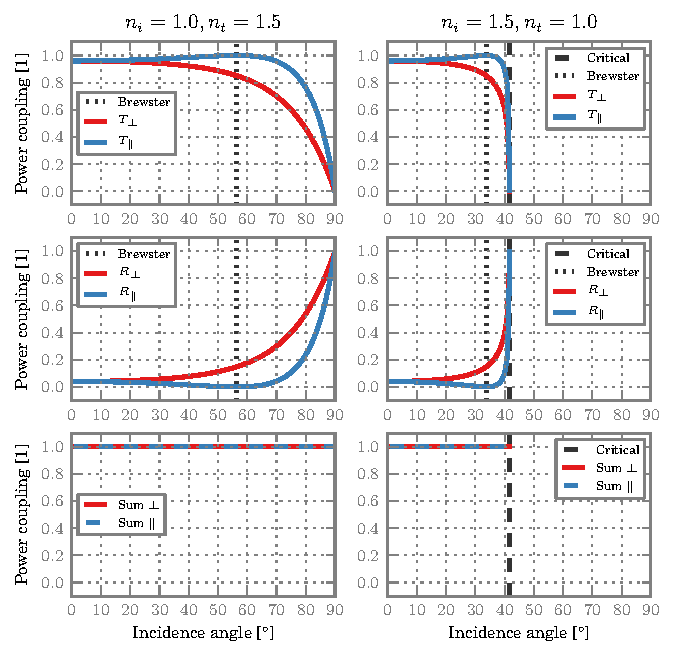
\includegraphics{interface_oblique_verification}
    \caption{Interface oblique, verification}
    \label{fig:interface_oblique_verification}
\end{figure}


%=============================================================================
\subsection{Thin film at normal incidence}
\label{sec:thin_film_at_normal_incidence}

%-----------------------------------------------------------------------------
\subsubsection{Scattering matrix}

Two interfaces separate three regions of space of refractive indices~$n_1$, $n_2$ and~$n_3$ (in most cases, $n_1=n_3$).
Each interface of the film reflects and transmits radiation according to the Fresnel equations for normal incidence~\eqref{eq:fresnel_normal}.
\Cref{fig:thin_film_normal} defines the notations for the reflection and transmission coeffients between the three regions of space.
The propagation between the two interfaces introduces a factor $a$.
\Cref{fig:thin_film_normal_collapsed} is what results of our modeling effort: a single network with two reflections and two transmissions.

\begin{figure}[hbtp]
    \centering
    \input{thin_film_normal.pdf_tex}
    \caption{Thin film at normal incidence.}
    \label{fig:thin_film_normal}
\end{figure}
\begin{figure}[hbtp]
    \centering
    \input{thin_film_normal_collapsed.pdf_tex}
    \caption{Thin film at normal incidence, collapsed.}
    \label{fig:thin_film_normal_collapsed}
\end{figure}

\Crefrange{eq:thin_film_normal_0}{eq:thin_film_normal_2} walk us through the derivation of~$r_{1, 3}$, the reflection coefficient of the thin film seen from the region of refractive index~$n_1$.
\begin{align}
    r_{1,3}
    &= r_{1,2} + t_{1,2}
        \left(
            a r_{2,3} a +
            a r_{2,3} a r_{2,1} a r_{2,3} a +
            \cdots
        \right)
       t_{2,1}
    \label{eq:thin_film_normal_0}
    \\
    r_{1, 3}
    &=
    r_{1, 2} + t_{1, 2} t_{2, 1} a^2r_{2, 3}
        \sum_{i=0}^{\infty} (a^2r_{2,1}r_{2,3})
    \label{eq:thin_film_normal_1}
    \\
    r_{1, 3}
    &=
    r_{1, 2} + t_{1, 2} t_{2, 1} a^2 r_{2, 3}
    \frac{1}{1 - a^2 r_{2, 1} r_{2, 3}}
    \label{eq:thin_film_normal_2}
\end{align}
Likewise, we can derive $r_{3, 1}$, $t_{1, 3}$ and $t_{3, 1}$.
They are given by \crefrange{eq:thin_film_normal_r31}{eq:thin_film_normal_t31},
with \cref{eq:thin_film_normal_r13} being a mere reminder of \cref{eq:thin_film_normal_2}.
\begin{subequations}
    \begin{align}
        r_{1, 3}
        &=
        r_{1, 2} + t_{1, 2} t_{2, 1} a^2 r_{2, 3}
        \frac{1}{1 - a^2 r_{2, 1} r_{2, 3}}
        \label{eq:thin_film_normal_r13}
        \\
        r_{3, 1}
        &=
        r_{3, 2} + t_{3, 2} t_{2, 3} a^2 r_{2, 1}
        \frac{1}{1 - a^2 r_{2, 3} r_{2, 1}}
        \label{eq:thin_film_normal_r31}
        \\
        t_{1, 3}
        &=
        t_{1,2} t_{2,3} a \frac{1}{1 - a^2 r_{2, 3} r_{2, 1}}
        \label{eq:thin_film_normal_t13}
        \\
        t_{3, 1}
        &=
        t_{3,2} t_{2,1} a \frac{1}{1 - a^2 r_{2, 1} r_{2, 3}}
        \label{eq:thin_film_normal_t31}
    \end{align}
\end{subequations}
The parameters $r_{1, 2}$, $t_{1, 2}$, $r_{3, 2}$, $t_{3, 2}$, $r_{2, 1}$, $t_{2, 1}$,
$r_{2, 3}$ and $t_{2, 3}$ are determined by the Fresnel equations for normal incidence~\eqref{eq:fresnel_normal}.
The parameter $a$ is determined by $\exp(-i 2 \pi d n f / c_0)$ according to \cref{eq:net_distance}.
Note that in these four equations, the fraction is the same;
it is sufficient to compute its value once only.



There is one more factor to apply: a compensation for the space taken by the film.
As illustrated in \cref{fig:thin_film_normal_compensation},
the film has a thickness $d_2$ and
its center is located at distances $d_1$ and $d_3$ from other reference points.
The actual length of the medium 1 is not $d_1$ but $d_1 - d_2/2$.
Likewise, the wave travels a distance $d_3 - d_2/2$ in the medium 3.
\begin{figure}[hbtp]
    \centering
    \input{thin_film_normal_compensation.pdf_tex}
    \caption{Thin film at normal incidence, space compensation.}
    \label{fig:thin_film_normal_compensation}
\end{figure}
One way of accounting for this without changing any other network is to add some negative space on each side of the film.
Let $a_1$ and $a_3$ be the effect of these negative spaces.
\Crefrange{eq:negative_space_3}{eq:negative_space_3} apply \cref{eq:net_distance} to the refractive indices $n_1$ and $n_3$ for the negative distance $-d_2/2$.
\begin{subequations}
    \begin{align}
        a_1 &= \exp \Big(-i 2 \pi (-d_2/2) n_1 f / c_0 \Big) \label{eq:negative_space_1}
        \\
        a_3 &= \exp \Big(-i 2 \pi (-d_2/2) n_3 f / c_0 \Big) \label{eq:negative_space_3}
    \end{align}
    \label{eq:negative_space}
\end{subequations}
The reflection on the left side crosses the negative space $a_1$ twice, therefore $r_{1, 3}$ must be multiplied by $a_1^2$.
Likewise, $r_{3, 1}$ must be multiplied by $a_3^2$.
Both transmissions $t_{1, 3}$ and $t_{3, 1}$ go through $a_1$ and $a_3$, therefore they must be multiplied by $a_1 a_3$.
This is summarized with \crefrange{eq:thin_film_normal_compensated_r13}{eq:thin_film_normal_compensated_t31}.
\begin{subequations}
    \begin{align}
        r'_{1, 3} &= a_1^2   \, r_{1, 3} \label{eq:thin_film_normal_compensated_r13} \\
        r'_{3, 1} &= a_3^2   \, r_{3, 1} \label{eq:thin_film_normal_compensated_r31} \\
        t'_{1, 3} &= a_1 a_3 \, t_{1, 3} \label{eq:thin_film_normal_compensated_t13} \\
        t'_{3, 1} &= a_1 a_3 \, t_{3, 1} \label{eq:thin_film_normal_compensated_t31}
    \end{align}
    \label{eq:thin_film_normal_compensated}
\end{subequations}

From there, building the scattering matrix of the thin film is straightforward.
If we name $I_3$ the 3--by--3 identity matrix,
then the Jones matrices  \crefrange{eq:thin_film_normal_s11}{eq:thin_film_normal_s22}
are the elements of the scattering matrix.
\begin{subequations}
    \begin{align}
        S_{1, 1} &= r'_{1, 3} I_3 \label{eq:thin_film_normal_s11} \\
        S_{1, 2} &= t'_{3, 1} I_3 \label{eq:thin_film_normal_s12} \\
        S_{2, 1} &= t'_{1, 3} I_3 \label{eq:thin_film_normal_s21} \\
        S_{2, 2} &= r'_{3, 1} I_3 \label{eq:thin_film_normal_s22}
    \end{align}
    \label{eq:thin_film_normal_sij}
\end{subequations}
If necessary, each of these Jones matrices can be adapted to account for the orientation of the thin film;
see~\vref{sec:rotating_jones_matrices}.

%-----------------------------------------------------------------------------
\subsubsection{Verification}
We have derived a model that treats a thin film as a single two-ports network.
It should yield the same results as a system of three networks
(interface--space--interface).
In this section, we verify this numerically.

\Cref{fig:thin_film_normal_verification_principle} defines the distances and refractive indices used in this section.
It also illustrates the two systems that we wish to compare:
\begin{itemize}
    \item one system made of three networks (two spaces, one thin film), that we call ``thin film model'';
    \item one system made of five networks (three spaces and two interfaces), that we call ``interfaces model''.
\end{itemize}
\begin{figure}[hbtp]
    \centering
    \input{thin_film_normal_verification_principle.pdf_tex}
    \caption{Thin film at normal incidence, verification, principle.}
    \label{fig:thin_film_normal_verification_principle}
\end{figure}

\Cref{fig:thin_film_normal_verification} presents the result of both models for
$n_1=1.00$, $n_2=1.75$, $n_3=1.50$,
$d_1=\SI{1}{\meter}$, $d_2=\SI{10}{\micro\meter}$ and $d_3=\SI{1}{\meter}$.
The source is on the leftmost port.
The ``Reflected'' plot corresponds to the output of that leftmost port.
The ``Transmitted'' plot corresponds to the output of the rightmost port.
\begin{figure}[hbtp]
    \centering
    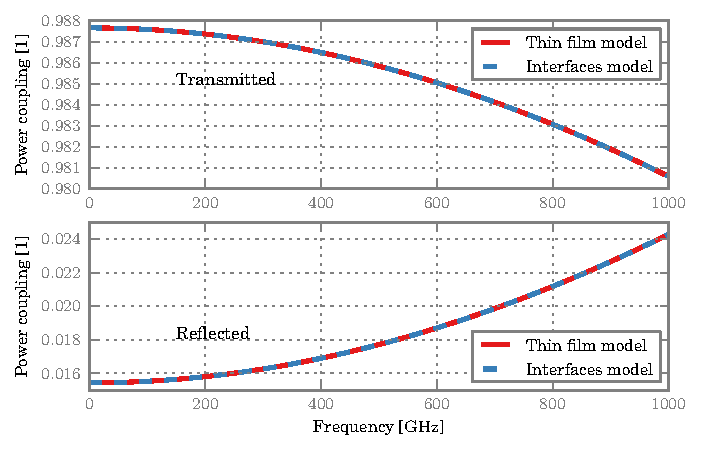
\includegraphics{thin_film_normal_verification.pdf}
    \caption{Thin film at normal incidence, verification.}
    \label{fig:thin_film_normal_verification}
\end{figure}

Both models agree within numerical noise.
The advantage of the thin film model over the other is that a thin film is represented by a single network.
This is easier for the programmer and faster for the computer.

The curvature of the power coupling displayed in \cref{fig:thin_film_normal_verification} comes from standing waves inside the thin film.
\Cref{eq:cavity_period} predicts a period of $F = c_0 / (2 n_2 d_2) \approx \SI{9993}{\tera\hertz}$.
Thin cavities (here \SI{10}{\micro\meter}) create standing wave patterns with very large periods.



%=============================================================================
\subsection{Thin film at oblique incidence}
\label{sec:thin_film_at_oblique_incidence}

A thin film at oblique incidence forms a four-ports network.
\Cref{fig:thin_film_oblique} defines the geometry and the port-numbering that we use.
\begin{figure}[hbtp]
    \centering
    \missingfigure{Thin film oblique}
    \caption{Thin film at oblique incidence}
    \label{fig:thin_film_oblique}
\end{figure}

When deriving the scattering matrix of a thin film at normal incidence in \cref{sec:thin_film_at_normal_incidence}, we allowed for three refractive indices: one for the film itself and one for each propagation medium on each side of the film.
This was a generalization that came at barely no cost because the geometry was simple.
In the case of a thin film at oblique incidence, we assume that the propagation medium on each side of the thin film has the same refractive index.
This is, after all, the most common case;
for example, a beam splitter placed in vacuum has vacuum on both sides.
If that constraint is too strong, it is always possible to model that thin film with three networks by using two interfaces and a distance (see sections~\ref{sec:generic_networks_distance} and \ref{sec:interface_at_oblique_incidence}).

%-----------------------------------------------------------------------------
\subsubsection{Geometry}
\label{sec:thin_film_geometry}
We need to determine the angle of incidence, the parallel and perpendicular decomposition matrices and the various rotation matrices.

It is assumed that we know the orientation of the thin film via its normal $n$ and the direction of propagation $k_1$ of the wave incident to the port 1.

From $n$ and $k_1$, we can apply \cref{eq:angle_from_dot_product} to compute the angle of incidence~$\theta_a$.
We get the refracted angle~$\theta_b$ from $\theta_a$ with \cref{eq:snell_thetab}.

We use \cref{eq:normal_to_plane_of_incidence} to retreive the normal to the plane of incidence $u$.

From the normal $u$ to the plane of incidence
and \cref{eq:para_perp_decomposition_matrix},
we determine the parallel and perpendicular projection matrices,
$M_\parallel$ and $M_\perp$.

From $u$ and
equations~\eqref{eq:quaternion_rotation_around_axis}
and \eqref{eq:quaternion_to_rotation_matrix}, we can compute the rotation matrices to apply to the Jones matrices and the direction of propagation.
The angles that we need are listed in \cref{eq:thin_film_angles}.
\begin{equation}
    \begin{aligned}
        \theta_{1 \leftarrow 2} &= 2 \theta_a
        &
        \theta_{2 \leftarrow 1} &= -2 \theta_a
        \\
        \theta_{3 \leftarrow 4} &= 2 \theta_a
        &
        \theta_{4 \leftarrow 3} &= -2 \theta_a
        \\
        \theta_{4 \leftarrow 1} &= -2 \theta_a
    \end{aligned}
    \label{eq:thin_film_angles}
\end{equation}
These angles $\theta_{i \leftarrow j}$ have corresponding rotation matrices $R^{i \leftarrow j}$.
We can already determine the directions of propagation of the waves exiting the thin film with \cref{eq:thin_film_propagation_rotation_ki}.
\begin{subequations}
    \begin{align}
        k_2 &= -R^{2 \leftarrow 1} k_1
        \label{eq:thin_film_propagation_rotation_k2}\\
        k_3 &= k_1
        \label{eq:thin_film_propagation_rotation_k3}\\
        k_4 &= R^{4 \leftarrow 1} k_1
        \label{eq:thin_film_propagation_rotation_k4}
    \end{align}
    \label{eq:thin_film_propagation_rotation_ki}
\end{subequations}

%-----------------------------------------------------------------------------
\subsubsection{Reflection and transmission coefficients}
In the previous section (\cref{sec:thin_film_geometry}) we have determined the decomposition and rotation matrices that are needed to compute the reflection and refraction coefficients of a thin film at oblique incidence.
We also have the angle of incidence and the refracted angle.

We want to apply the Fresnel equations for oblique incidence \eqref{eq:fresnel_oblique} twice:
once for entering the thin film, and once for leaving it.
\begin{itemize}
    \item 
$r_{\parallel a}$, $r_{\perp a}$, $t_{\parallel a}$ and $t_{\perp a}$ correspond to entering the film.
They are derived from \cref{eq:fresnel_oblique} with
$\theta_i = \theta_a$, $\theta_t = \theta_b$,
$n_i = n_a$ and $n_t = n_b$.
    \item
$r_{\parallel b}$, $r_{\perp b}$, $t_{\parallel b}$ and $t_{\perp b}$ correspond to exiting the film.
They are derived from \cref{eq:fresnel_oblique} with
$\theta_i = \theta_b$, $\theta_t = \theta_a$,
$n_i = n_b$ and $n_t = n_a$.
\end{itemize}

The pathlength $l_b$ inside the film is not equal to the thickness $d$ of the thin film because $\theta_b \ne 0$, as described by \cref{eq:thin_film_oblique_pathlength}.
\begin{equation}
    l_b = \frac{d}{\cos \theta_b}
    \label{eq:thin_film_oblique_pathlength}
\end{equation}
To this distance $l_b$ corresponds a gain $a_b$ that we derive from \cref{eq:net_distance}.
Its expression is given for $l_b$ in \cref{eq:thin_film_distance}.
\begin{equation}
    a_b = \exp(-2i \pi l_b n_b f / c_0)
    \label{eq:thin_film_distance}
\end{equation}
This pathlength $l_b$ must be compensated for.
Indeed, the pathlength $l_b$ inside the film replaces a pathlength $l_a$ in the material $n_a$.
\begin{equation}
    l_a = \frac{d}{\cos \theta_a}
    \label{eq:thin_film_oblique_pathlength_compensation}
\end{equation}
\begin{equation}
    a_a = \exp(-2i \pi (-l_a) n_a f / c_0)
    \label{eq:thin_film_distance_compensation}
\end{equation}

What follows is similar to what we did for the thin film at normal incidence.
One difference is that do it twice, one for the parallel parameters and one for the perpendicular parameters.
Another difference is that we have two and not three refractive indices, which gives a few simplifications.
\begin{subequations}
    \begin{align}
        t_\parallel
        &=
        a_a \,
        t_{\parallel a} \, t_{\parallel b} \, a_b
        \frac{1}{
            1 - (r_{\parallel b} \, a_b)^2
        }
        \\
        t_\perp
        &=
        a_a \,
        t_{\perp a} \, t_{\perp b} \, a_b
        \frac{1}{
            1 - (r_{\perp b} \, a_b)^2
        }
        \\
        r_\parallel
        &=
        a_a \,
        r_{\parallel a} + r_{\parallel b} \, a_b \, t_\parallel
        \\
        r_\perp
        &=
        a_a \,
        r_{\perp a} + r_{\perp b} \, a_b \, t_\perp
    \end{align}
\end{subequations}

\subsubsection{Scattering matrix}
Because we use one refractive index only outside the film, the transmitted waves are not rotated.
\begin{equation}
    S_{1, 3} =
    S_{2, 4} =
    S_{3, 1} =
    S_{4, 2} =
    t_\parallel M_\parallel
    +
    t_\perp M_\perp
    \label{eq:thin_film_s_t}
\end{equation}

The reflections, however, require some rotations.
\begin{subequations}
    \begin{align}
        S_{1, 2} = R^{1 \leftarrow 2} (r_\parallel M_\parallel + r_\perp M_\perp) \\
        S_{2, 1} = R^{2 \leftarrow 1} (r_\parallel M_\parallel + r_\perp M_\perp) \\
        S_{3, 4} = R^{3 \leftarrow 4} (r_\parallel M_\parallel + r_\perp M_\perp) \\
        S_{4, 3} = R^{4 \leftarrow 3} (r_\parallel M_\parallel + r_\perp M_\perp)
    \end{align}
    \label{eq:thin_film_s_r}
\end{subequations}

Finally, many paths are forbidden.
\begin{equation}
    S_{1, 1} = S_{1, 4} = S_{2, 2} = S_{2, 3} =
    S_{3, 2} = S_{3, 3} = S_{4, 1} = S_{4, 4} = 
    \begin{pmatrix}
        0&0&0\\0&0&0\\0&0&0
    \end{pmatrix}
    \label{eq:thin_film_s_zero}
\end{equation}

\Crefrange{eq:thin_film_s_t}{eq:thin_film_s_zero} define the scattering parameters of the 4--by--4 scattering matrix of a thin film at oblique incidence.


\subsubsection{Verification}
Our model for a thin film at oblique incidence should provide exactly the same result as two interfaces and a distance.
The goal of the thin film model is to provide convenience, not introduce new physics.
\Cref{fig:thin_film_oblique_verification} illustrates a comparison between these two ways of modeling a thin film.
The angle of incidence is~\SI{45}{\degree}.
The film is~\SI{10}{\micro\meter} thick.
The refractive indices are 1.0 outside the film and 1.5 in the film.
The thickness of the film creates a cavity and therefore a standing wave.
This standing wave is responsable for the frequency-dependance of the reflected and transmitted power seen on \cref{fig:thin_film_oblique_verification}.

\begin{figure}[hbtp]
    \centering
    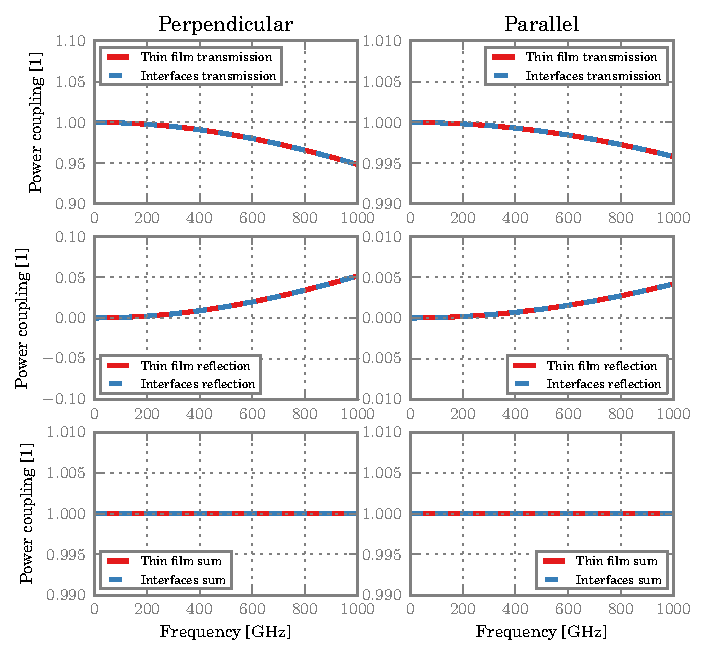
\includegraphics{thin_film_oblique_verification}
    \caption{Thin film oblique, verification}
    \label{fig:thin_film_oblique_verification}
\end{figure}

The top row of \cref{fig:thin_film_oblique_verification} shows the transmitted power, the middle row shows the reflected power, and the bottom row shows the sum of the two.
That last row shows that energy is conserved: the power that is not transmitted is reflected.

The left column shows the transmitted, reflected and total power coupling for the perpendicular polarization.
The right column corresponds to the parallel polarization.
Note that the vertical-axes differ for the two polarizations: the standing wave has an effect about ten times stronger on the perpendicular polarization.

Finally, each plot shows two overlapped curves.
The red curve corresponds to the model derived in this section with which the thin film is seen as a single network.
The blue curve corresponds to a model made of two interfaces and a distance.

As expected, both models agree within numerical noise.
This agreement does not only happen in power, but also in field.
The phasor predicted by both methods agree within $10^{-10}$: the magnitude of the difference of the phasors is smaller than $10^{-10}$ for frequencies of the order of \SI{1}{\tera\hertz}.  \todo{Should I put a pic?}



%=============================================================================
\subsection{Wire grid polarizer}
\todo{Check k omega convention}
In their paper from \citeyear{houde_2001} \citetitle{houde_2001}, \textcite{houde_2001} present a set of equations that approximate the electric field at any point near a wire grid polarizer.
The incident wave is assumed plane, the surrounding propagation medium is assumed homogeneous and isotropic, and the wires are assumed to be free floating (no dielectric substrate) and to have a cylindrical section.

\subsubsection{Geometry}
The article of \citeauthor{houde_2001} \cite{houde_2001} defines the following rest reference frame for the grid: wires in the $\vect{x}\vect{y}$ plane, wires along $\vect{x}$.
Its normal, at rest, is therefore the $\vect{z}$ axis.

If $R$ is the rotation matrix that move the grid from its rest attitude to its useful attitude, then the normal of the grid is $\vect{n}=R \vect{z}$.

The grid is a four port network.
$\vect{k}_1$,  is the direction of propagation of the wave indident to the port 1.
We can derive the direction of propagation of the wave incident to the three other ports easily.
The law of reflection states that $\vect{k}_1$, $\vect{k}_2$ and $\vect{n}$ are coplanar and that the directed angle between $\vect{k}_1$ and $\vect{n}$ equals that between $\vect{n}$ and $\vect{k}_2$.
Therefore, one way of deriving $\vect{k}_2$ is to rotate $\vect{k}_1$ by \SI{180}{\degree} around $\vect{n}$.
Then, $\vect{k}_3=-\vect{k}_1$ and $\vect{k}_4=-\vect{k_2}$.

\subsubsection{Reflection and transmission coefficients}
The set of equations that interest us here are the equations numbered 23 to 35, 62 and 63 in the article of \citeauthor{houde_2001} \cite{houde_2001}, which we copied here for convenience.
The first two equations, \eqref{eq:grid_current_linear} and \eqref{eq:grid_current_circular}, describe the electric current in the wires.
$K^x$ corresponds to a linear current and $K^\theta$ to a circular current.
In the first case, electrons move along the length of the wire; in the other, they rotate around the axis of the wire.
\begin{align}
    K^x &= \frac{E_0}{F} \cdot \alpha' \frac{N_x}{\Delta_x}
    \label{eq:grid_current_linear}
    \\
    K^\theta &= (-j) \frac{E_0}{F} \cdot (\gamma' \beta - \beta' \gamma) \frac{N_\theta}{\Delta_\theta}
    \label{eq:grid_current_circular}
\end{align}
with
\begin{align}
    N_x
    &=
    1 - j \frac{Z_s}{Z_0} \frac{ka}{2}
    \\
    \Delta_x
    &=
    (1 - \alpha^2) S_1 - j \frac{Z_s}{Z_0} \sqrt{1 - \alpha^2}H_1^{(2)} (k'a)
    \\
    N_\theta
    &=
    1 + j \frac{Z_s}{Z_0} \frac{2}{ka}
    \\
    \Delta_\theta
    &=
    \sqrt{1 - \alpha^2} H_1^{(2)} (k'a) + j \frac{Z_s}{Z_0} (1 - \alpha^2) S_1
\end{align}
and
\begin{equation}
    S_1 = H_0^{(2)} (k'a) + 2
    \sum_{n=1}^\infty
    H_0^{(2)}(k'nd) \cos (k \beta nd)
    \text{.}
    \label{eq:infinite_hankel}
\end{equation}
The following equations use the previous definitions.
They describe the reflected and transmitted fields in three dimensions for a grid in the $xy$-plane, wires along~$x$.
\begin{align}
    R^x
    &=
    -\frac{F}{E_0}
    \frac{\lambda}{\pi d}
    \frac{1 - \alpha^2}{\gamma} K^x
    \label{eq:houde_Rx}
    \\
    R^y
    &=
    \phantom{-}
    \frac{F}{E_0}
    \frac{\lambda}{\pi d}
    \left[
        \frac{\alpha \beta}{\gamma} K^x
        -
        j \frac{ka}{2} K^\theta
    \right]
    \\
    R^z
    &=
    -\frac{F}{E_0}
    \frac{\lambda}{\pi d}
    \left[
       \alpha K^x
       +
       j \frac{\beta}{\gamma} \frac{ka}{2} K^\theta
    \right]
    \\
    T^x &= \alpha' + R^x
    \\
    T^y
    &=
    \beta' +
    \frac{F}{E_0}
    \frac{\lambda}{\pi d}
    \left[
        \frac{\alpha \beta}{\gamma} K^x + j \frac{ka}{2} K^\theta
    \right]
    \\
    T^z
    &=
    \gamma' +
    \frac{F}{E_0}
    \frac{\lambda}{\pi d}
    \left[
        \alpha K^x - j \frac{\beta}{\gamma} \frac{ka}{2} K^\theta
    \right]
\end{align}
Note that Houde calls these $R$ and $T$ ``reflection'' and ``transmission coefficient'', something they are not quite since they contain $\alpha'$, $\beta'$ and $\gamma'$, corresponding to the amplitude of the incoming electric field in the three dimensions.
These amplitudes have to be factored out if we want to really speak about reflection or transmission coefficients.

When implementing these equations, some simplifications are obvious.
For example, $\frac{E_0}{F}$ inside $K^x$ and $K^\theta$ cancels $\frac{F}{E_0}$ in $R$ and $T$;
the complex unit $j$ within $K^\theta$ combines with $j$ in $R$ and $T$ to become -1.

In these equations, $\alpha'$, $\beta'$ and $\gamma'$ are the three components of the direction of the incident electric field, satisfying $\alpha'^2 + \beta'^2 + \gamma'^2 = 1$.
That condition seems to apply only to real numbers, restricting the use of this grid model to waves that are linearly polarized (their three components are in phase).
However, there is no such limitation in the model.
Indeed, the authors define the incident electric field as $(e_x, e_y, e_z) = E_0(\alpha', \beta', \gamma')$.
The amplitude $E_0$ can be complex and it seems that its phase has to be shared among the three components.
However, when we rewrite the equations to fit in a matrix, we will notice that the real parameters are not $\alpha'$, $\beta'$, $\gamma'$ and $E_0$, but $e_x$, $e_y$ and $e_z$ directly, which are all independant.
In that case, each of them is free to have its own phase and the model also applies to elliptically polarized waves.


In order to rewrite these equations in a matrix form that depends on $e_x$, $e_y$ and $e_z$, one needs to split each coefficient of transmission and reflection into three, like this:
\begin{equation}
    e_{rx} = R^{xx} e_x + R^{xy} e_y + R^{xz} e_z
\end{equation}
so that we can write
\begin{align}
    e_r &= R e_i \\
    e_r &=
    \begin{pmatrix}
        R_{xx} & R_{xy} & R_{xz} \\
        R_{yx} & R_{yy} & R_{yz} \\
        R_{zx} & R_{zy} & R_{zz}
    \end{pmatrix}
    e_i
\end{align}
for the reflection $R$ and a similar equation for the transmission $e_t = T e_i$.
I start with $R_x$ defined in \cref{eq:houde_Rx} to get $R_{xx}$, $R_{xy}$ and $R_{xz}$.
\begin{align*}
    e_{rx} &= R^x E_0
    \\
           &= -\frac{F}{E_0}
              \frac{\lambda}{\pi d}
              \frac{1-\alpha^2}{\gamma}
              K^x
              E_0
    \\
           &= -\cancel{\frac{F}{E_0}}
              \frac{\lambda}{\pi d}
              \frac{1-\alpha^2}{\gamma}
              \cancel{\frac{E_0}{F}}
              \frac{N_x}{\Delta_x}
              \underbrace{
                  \alpha'
                  E_0
              }_{e_{ix}}
    \\
           &= -\frac{\lambda}{\pi d}
              \frac{1-\alpha^2}{\gamma}
              \frac{N_x}{\Delta_x}
              e_{ix}
\end{align*}
By identification, we find these values for $R_{xx}$, $R_{xy}$ and $R_{xz}$.
\begin{equation}
    \left\lbrace
    \begin{aligned}
        R_{xx} &= -\frac{\lambda}{\pi d}
                  \frac{N_x}{\Delta_x}
                  \frac{1-\alpha^2}{\gamma}
        \\
        R_{xy} &= 0
        \\
        R_{xz} &= 0
    \end{aligned}
    \right.
\end{equation}
Let us continue with $R_y$.
\begin{align*}
    e_{ry}
    &= R^y E_0
    \\
    &= \frac{F}{E_0}
       \frac{\lambda}{\pi d}
       \left[
           \frac{\alpha \beta}{\gamma}
           K^x
           -
           j
           \frac{ka}{2}
           K^\theta           
       \right]
       E_0
    \\
    &= \cancel{\frac{F}{E_0}}
       \frac{\lambda}{\pi d}
       \left[
           \frac{\alpha \beta}{\gamma}
           \cancel{\frac{E_0}{F}}
           \frac{N_x}{\Delta_x}
           \alpha'
           -
           j
           \frac{ka}{2}
           (-j)
           \cancel{\frac{E_0}{F}}
           \frac{N_\theta}{\Delta_\theta}
           (\gamma' \beta - \beta' \gamma)           
       \right]
       E_0
    \\
    &= \frac{\lambda}{\pi d}
       \left[
           \frac{\alpha \beta}{\gamma}
           \frac{N_x}{\Delta_x}
           \alpha'
           +
           \frac{ka}{2}
           \frac{N_\theta}{\Delta_\theta}
           \gamma
           \beta'
           -
           \frac{ka}{2}
           \frac{N_\theta}{\Delta_\theta}
           \beta
           \gamma'
       \right]
       E_0
    \\
    &= \frac{\lambda}{\pi d}
       \frac{\alpha \beta}{\gamma}
       \frac{N_x}{\Delta_x}
       \underbrace{E_0 \alpha'}_{e_{ix}}
       +
       \frac{\lambda}{\pi d}
       \frac{ka}{2}
       \frac{N_\theta}{\Delta_\theta}
       \gamma
       \underbrace{E_0 \beta'}_{e_{iy}}
       -
       \frac{\lambda}{\pi d}
       \frac{ka}{2}
       \frac{N_\theta}{\Delta_\theta}
       \beta
       \underbrace{E_0 \gamma'}_{e_{iz}}
\end{align*}
\begin{equation}
    \left\lbrace
    \begin{aligned}
        R_{yx}
        &=
        \phantom{-}
        \frac{\lambda}{\pi d}
        \frac{N_x}{\Delta_x}
        \frac{\alpha \beta}{\gamma}
        \\
        R_{yy}
        &=
        \phantom{-}
        \frac{\lambda}{\pi d}
        \frac{N_\theta}{\Delta_\theta}
        \frac{ka}{2}
        \gamma
        \\
        R_{yz}
        &=
        -
        \frac{\lambda}{\pi d}
        \frac{N_\theta}{\Delta_\theta}
        \frac{ka}{2}
        \beta
    \end{aligned}
    \right.
\end{equation}
Same thing for $R_z$.
\begin{align*}
    e_{rz} &= R^z E_0
    \\
    &=
    -
    \frac{F}{E_0}
    \frac{\lambda}{\pi d}
    \left[
        \alpha K^x
        +
        j
        \frac{\beta}{\gamma}
        \frac{ka}{2}
        k^\theta
    \right]
    E_0
    \\
    &=
    -
    \cancel{\frac{F}{E_0}}
    \frac{\lambda}{\pi d}
    \left[
        \alpha
        \cancel{\frac{E_0}{F}}
        \frac{N_x}{\Delta_x}
        \alpha'
        +
        j
        \frac{\beta}{\gamma}
        \frac{ka}{2}
        (-j)
        \cancel{\frac{E_0}{F}}
        (\gamma' \beta - \beta' \gamma)
        \frac{N_\theta}{\Delta_\theta}
    \right]
    E_0
    \\
    &=
    -
    \frac{\lambda}{\pi d}
    \alpha
    \frac{N_x}{\Delta_x}
    \underbrace{E_0 \alpha'}_{e_{ix}}
    +
    \frac{\lambda}{\pi d}
    \frac{\beta}{\gamma}
    \frac{ka}{2}
    \frac{N_\theta}{\Delta_\theta}
    \gamma
    \underbrace{E_0 \beta'}_{e_{iy}}
    -
    \frac{\lambda}{\pi d}
    \frac{\beta}{\gamma}
    \frac{ka}{2}
    \frac{N_\theta}{\Delta_\theta}
    \beta
    \underbrace{E_0 \gamma'}_{e_{iz}}
\end{align*}
\begin{equation}
    \left\lbrace
    \begin{aligned}
        R_{zx}
        &=
        -
        \frac{\lambda}{\pi d}
        \frac{N_x}{\Delta_x}
        \alpha
        \\
        R_{zy}
        &=
        \phantom{-}
        \frac{\lambda}{\pi d}
        \frac{N_\theta}{\Delta_\theta}
        \frac{ka}{2}
        \beta
        \\
        R_{zz}
        &=
        -
        \frac{\lambda}{\pi d}
        \frac{N_\theta}{\Delta_\theta}
        \frac{ka}{2}
        \frac{\beta^2}{\gamma}
    \end{aligned}
    \right.
\end{equation}
We have the reflection matrix.
Now, we compute the transmission matrix.
\begin{align*}
    e_{tx} &= T^x E_0
    \\
    &= (\alpha' + R^x) E_0
    \\
    &= \underbrace{\alpha' E_0}_{e_{ix}}
       -
       \frac{\lambda}{\pi d}
       \frac{1 - \alpha^2}{\gamma}
       \frac{N_x}{\Delta_x}
       \underbrace{\alpha' E_0}_{e_{ix}}
    \\
    &= \left(
           1
           -
           \frac{\lambda}{\pi d}
           \frac{1 - \alpha^2}{\gamma}
           \frac{N_x}{\Delta_x}
       \right)
       e_{ix}
\end{align*}
\begin{equation}
    \left\lbrace
    \begin{aligned}
        T_{xx}
        &= 1
           -
           \frac{\lambda}{\pi d}
           \frac{N_x}{\Delta_x}
           \frac{1 - \alpha^2}{\gamma}
        \\
        T_{xy} &= 0
        \\
        T_{xz} &= 0
    \end{aligned}
    \right.
\end{equation}

\begin{align*}
    e_{ty} &= T^y E_0
    \\
    &=
    \left(
        \beta'
        +
        \frac{F}{E_0}
        \frac{\lambda}{\pi d}
        \left[
            \frac{\alpha \beta}{\gamma}
            K^x
            +
            j
            \frac{ka}{2}
            K^\theta
        \right]
    \right)
    E_0
    \\
    &=
    \left(
        \beta'
        +
        \cancel{\frac{F}{E_0}}
        \frac{\lambda}{\pi d}
        \left[
            \frac{\alpha \beta}{\gamma}
            \cancel{\frac{E_0}{F}}
            \frac{N_x}{\Delta_x}
            \alpha'
            +
            j
            \frac{ka}{2}
            (-j)
            \cancel{\frac{E_0}{F}}
            \frac{N_\theta}{\Delta_\theta}
            (\gamma' \beta - \beta' \gamma)
        \right]
    \right)
    E_0
    \\
    &=
    \left(
        \beta'
        +
        \frac{\lambda}{\pi d}
        \frac{\alpha \beta}{\gamma}
        \frac{N_x}{\Delta_x}
        \alpha'
        -
        \frac{\lambda}{\pi d}
        \frac{ka}{2}
        \frac{N_\theta}{\Delta_\theta}
        \gamma
        \beta'
        +
        \frac{\lambda}{\pi d}
        \frac{ka}{2}
        \frac{N_\theta}{\Delta_\theta}
        \beta
        \gamma'
    \right)
    E_0
    \\
    &=
    \frac{\lambda}{\pi d}
    \frac{\alpha \beta}{\gamma}
    \frac{N_x}{\Delta_x}
    \underbrace{E_0 \alpha'}_{e_{ix}}
    +
    \left(
        1
        -
        \frac{\lambda}{\pi d}
        \frac{ka}{2}
        \frac{N_\theta}{\Delta_\theta}
        \gamma
    \right)
    \underbrace{E_0 \beta'}_{e_{iy}}
    +
    \frac{\lambda}{\pi d}
    \frac{ka}{2}
    \frac{N_\theta}{\Delta_\theta}
    \beta
    \underbrace{E_0 \gamma'}_{e_{iz}}
\end{align*}
\begin{equation}
    \left\lbrace
    \begin{aligned}
        T_{yx}
        &= \frac{\lambda}{\pi d}
           \frac{N_x}{\Delta_x}
           \frac{\alpha \beta}{\gamma}
        \\
        T_{yy}
        &= 1
           -
           \frac{\lambda}{\pi d}
           \frac{N_\theta}{\Delta_\theta}
           \frac{ka}{2}
           \gamma
        \\
        T_{yz}
        &= \frac{\lambda}{\pi d}
           \frac{N_\theta}{\Delta_\theta}
           \frac{ka}{2}
           \beta
    \end{aligned}
    \right.
\end{equation}

\begin{align*}
    e_{tz} &= T^z E_0
    \\
    &=
    \left(
        \gamma' +
        \frac{F}{E_0}
        \frac{\lambda}{\pi d}
        \left[
            \alpha K^x - j \frac{\beta}{\gamma} \frac{ka}{2} K^\theta
        \right]
    \right)
    E_0
    \\
    &=
    \left(
        \gamma' +
        \cancel{\frac{F}{E_0}}
        \frac{\lambda}{\pi d}
        \left[
            \alpha
            \cancel{\frac{E_0}{F_0}}
            \frac{N_x}{\Delta_x}
            \alpha'
            -
            j
            \frac{\beta}{\gamma}
            \frac{ka}{2}
            (-j)
            \cancel{\frac{E_0}{F}}
            \frac{N_\theta}{\Delta_\theta}
            (\gamma' \beta - \beta' \gamma)
        \right]
    \right)
    E_0
    \\
    &=
    \left(
        \gamma' +
        \frac{\lambda}{\pi d}
        \left[
            \alpha
            \frac{N_x}{\Delta_x}
            \alpha'
            +
            \frac{\beta}{\gamma}
            \frac{ka}{2}
            \frac{N_\theta}{\Delta_\theta}
            \gamma
            \beta'
            -
            \frac{\beta}{\gamma}
            \frac{ka}{2}
            \frac{N_\theta}{\Delta_\theta}
            \beta
            \gamma'
        \right]
    \right)
    E_0
    \\
    &=
    \frac{\lambda}{\pi d}
    \alpha
    \frac{N_x}{\Delta_x}
    \underbrace{E_0 \alpha'}_{e_{ix}}
    +
    \frac{\lambda}{\pi d}
    \frac{\beta}{\gamma}
    \frac{ka}{2}
    \frac{N_\theta}{\Delta_\theta}
    \gamma
    \underbrace{E_0 \beta'}_{e_{iy}}
    +
    \left(
        1
        -
        \frac{\lambda}{\pi d}
        \frac{\beta}{\gamma}
        \frac{ka}{2}
        \frac{N_\theta}{\Delta_\theta}
        \beta
    \right)
    \underbrace{E_0 \gamma'}_{e_{iz}}
\end{align*}
\begin{equation}
    \left\lbrace
    \begin{aligned}
        T_{zx}
        &= \frac{\lambda}{\pi d}
           \frac{N_x}{\Delta_x}
           \alpha
        \\
        T_{zy}
        &= \frac{\lambda}{\pi d}
           \frac{N_\theta}{\Delta_\theta}
           \frac{ka}{2}
           \frac{\beta}{\gamma}
           \gamma
        \\
        T_{zz}
        &= 1
           -
           \frac{\lambda}{\pi d}
           \frac{N_\theta}{\Delta_\theta}
           \frac{ka}{2}
           \frac{\beta}{\gamma}
           \beta
    \end{aligned}
    \right.
\end{equation}

Another simplification:
\begin{equation}
    k = 2\pi / \lambda
    \quad \Rightarrow \quad
    \frac{\lambda}{\pi d} \frac{ka}{2}
    =
    \frac{\lambda}{\pi d} \frac{2\pi a}{2\lambda}
    =
    \frac{a}{d}
\end{equation}

\begin{equation}
    R =
    \begin{pmatrix}
        -\frac{\lambda}{\pi d}
        \frac{N_x}{\Delta_x}
        \frac{1 - \alpha^2}{\gamma}
        &
        0
        &
        0
        \\
        \frac{\lambda}{\pi d}
        \frac{N_x}{\Delta_x}
        \frac{\alpha \beta}{\gamma}
        &
        \frac{\lambda}{\pi d}
        \frac{N_\theta}{\Delta_\theta}
        \frac{ka}{2}
        \gamma
        &
        -
        \frac{a}{d}
        \frac{N_\theta}{\Delta_\theta}
        \beta
        \\
        -
        \frac{\lambda}{\pi d}
        \frac{N_x}{\Delta_x}
        \alpha
        &
        \frac{a}{d}
        \frac{N_\theta}{\Delta_\theta}
        \beta
        &
        -
        \frac{a}{d}
        \frac{N_\theta}{\Delta_\theta}
        \frac{\beta^2}{\gamma}
    \end{pmatrix}
\end{equation}
\begin{equation}
    T =
    \begin{pmatrix}
        1 -
        \frac{\lambda}{\pi d}
        \frac{N_x}{\Delta_x}
        \frac{1 - \alpha^2}{\gamma}
        &
        0
        &
        0
        \\
        \frac{\lambda}{\pi d}
        \frac{N_x}{\Delta_x}
        \frac{\alpha \beta}{\gamma}
        &
        1 -
        \frac{a}{d}
        \frac{N_\theta}{\Delta_\theta}
        \gamma
        &
        \frac{a}{d}
        \frac{N_\theta}{\Delta_\theta}
        \beta
        \\
        \frac{\lambda}{\pi d}
        \frac{N_x}{\Delta_x}
        \alpha
        &
        \frac{a}{d}
        \frac{N_\theta}{\Delta_\theta}
        \beta
        &
        1 -
        \frac{a}{d}
        \frac{N_\theta}{\Delta_\theta}
        \frac{\beta^2}{\gamma}
    \end{pmatrix}
\end{equation}
These reflection and transmission matrices are Jones matrices.
The parameters are the radius $a$ of the wires,
the distance $d$ between the wires,
the conductivity $\sigma$ of the wires,
the frequency $f$ of the wave and
the direction of propagation $\vect{k_1}=(\alpha, \beta, \gamma)$.
We could consider the impedance of the surrounding medium as an additional parameter instead of using that of vacuum, but we did not need that.

\subsubsection{Scattering matrices}
The reflection and transmission matrices defined above are Jones matrices.
But before, we must apply rotation matrices to them in order to account for the arbitrary orientation of the grid.
Indeed, these Jones matrices are valid for grid lying in the $(x, y)$ plane, with the wires along $x$.






%#############################################################################

\section{Simple systems}
\label{sec:simple_systems}

The idea is to show that it works and makes sense.



%=============================================================================

\subsection{The simplest cavity}
\label{sec:the_simplest_cavity}

\Cref{fig:simple_cavity_principle} illustrates how three networks can represent a simple cavity: two interfaces separated by some space.
The three networks all have two ports numbered according to \cref{fig:simple_cavity_principle}.
Ports 2 and 3 are coupled, and so are ports 4 and 5.
Ports 1 and 6 are open to the outside world.

\begin{figure}[hbtp]
    \centering
    \input{simple_cavity_principle.pdf_tex}
    \caption{Simple cavity, principle.}
    \caption*{
        Two reflective surfaces facing each other form a cavity.
        Here, the surfaces are defined by the interfaces (vertical dotted lines)
        between regions of space of different refractive indices $n_1$ and $n_2$.
        According to the Fresnel equations~\eqref{eq:fresnel_normal}, these interfaces
        reflect and transmit part of the incident radiation (black arrows).
        As a result, a standing wave is formed inside the cavity.
        That standing wave is the superposition of an infinity of traveling waves
        interfering with each other.
        We can model such a system with three two-ports networks:
        one for each interface and one for the space between them.
        The numbers 1 to~6 are our arbitrary labels for the ports.
    }
    \label{fig:simple_cavity_principle}
\end{figure}
\begin{figure}[hbtp]
    \centering
    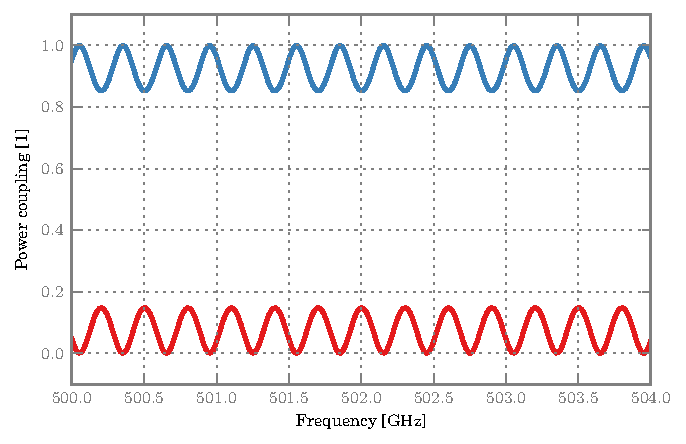
\includegraphics{simple_cavity_direct}
    \caption{Simple cavity, model result.}
    \caption*{
        The blue curve, on top, corresponds to the power coupling of port~6,
        that is the transmission through the cavity.
        The red curve, on the bottom, corresponds to the power coupling of port~1,
        that is the reflection on the cavity.
    }
    \label{fig:simple_cavity_direct}
\end{figure}
\begin{figure}[hbtp]
    \centering
    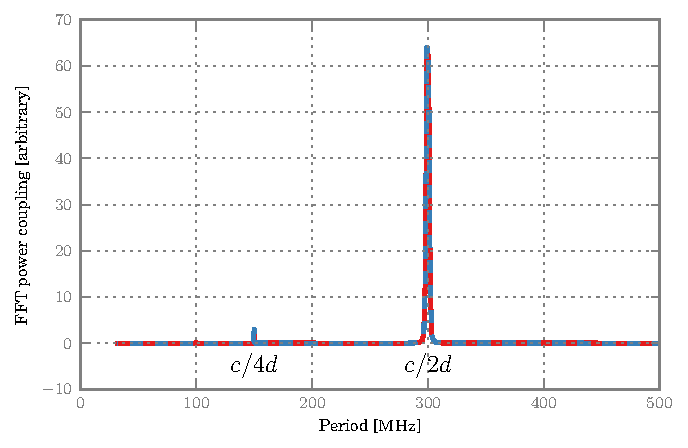
\includegraphics{simple_cavity_fft}
    \caption{Simple cavity, Fourier transform of the model result.}
    \caption*{
        The transmitted (blue) and reflected (red) wave show the same amount of modulation
        introduced by the cavity.
        The fundamental is at a period $F=c/2d$ with $c$ the speed of light in the cavity
        and $d$ the length of the cavity.
        An harmonic shows at $F=c/4d$,
        proving that the modulation is not perfectly sinusoidal.
        This spectrum was obtained by running the model for 4001 frequencies
        over a~\SI{64}{\giga\hertz} range,
        multiplying the result by a hanning window and taking a fast Fourier transform.
    }
    \label{fig:simple_cavity_fft}
\end{figure}

\Cref{fig:simple_cavity_direct} presents the result of the model for the following parameters:
\begin{itemize}
    \item refractive index $n_1=1.5$,
    \item refractive index $n_2=1.0$,
    \item distance between the interfaces $d=\SI{0.5}{\meter}$,
    \item frequency $f$ from \SIrange{500}{504}{\giga\hertz}.
\end{itemize}
The scattering matrices of the interfaces are derived from~\vref{eq:s_interface_normal} using $n_1$ and $n_2$.
The scattering matrix of the space between the interfaces is derived from~\vref{eq:scattering_distance} using $d$, $n_1$ and $f$.



%-----------------------------------------------------------------------------

\subsubsection{Periodicity}
According to \cref{eq:cavity_period}, we expect a periodicity of $F=c/2d$ where $c=c_0/n$ is the speed of light in the cavity and $d$ the length of the cavity.
With $c_0\approx \SI{2.998e8}{\meter\per\second}$, $n=1$ and $d=\SI{0.5}{\meter}$, we get $F \approx \SI{299.8}{\mega\hertz}$.

Our model agrees with our expectation, as shown by the fourrier transform in \cref{fig:simple_cavity_fft}.



%-----------------------------------------------------------------------------

\subsubsection{Energy conservation}
Examination of the results displayed in \cref{fig:simple_cavity_direct} reveals that energy is neither created nor destroyed.
The power is always positive, and the sum of the transmitted (blue) and reflected (red) power always equal 1 within numerical noise.
The power that is not transmitted through the cavity is reflected back to the source.



%=============================================================================

\subsection{Thin film beam splitter}

A thin dielectric film can be used as a beam splitter, as illustrated in \cref{fig:beam_splitter_principle}.
\begin{figure}[hbtp]
    \centering
    \input{beam_splitter_principle.pdf_tex}
    \caption{Beam splitter, principle.}
    \label{fig:beam_splitter_principle}
\end{figure}

This setup is one of the simplest way to inject local oscillator (LO) and sky signal together on a mixer.
What we have here is a heterodyne telescope.
The very transparent thin film couples most of the sky signal to the mixer, while coupling almost none of the local oscillator noise.
Unfortunately, the thin film is also transparent to the LO signal (narrow line at the LO frequency) required to pump the mixer, so the LO signal must be very strong.
This design wastes most of the LO power but has the advantage of being simple.
HIFI uses a similar approach for its bands 1, 2 and 3 (with wire grid polarizers instead of thin films though).

%-----------------------------------------------------------------------------

\subsubsection{Modeling the networks}

We can model the thin film using the principle described in \cref{sec:thin_film_at_oblique_incidence}.
Let us model a thin film of biaxially-oriented polyethylene terephthalate or ``boPET'', more commonly known under trade-mame ``Mylar''.
The table entry for ``PETP'' in the article of \citeauthor{lamb1996miscellaneous}~\cite{lamb1996miscellaneous} suggests that we choose 1.83 for the refractive index of the film at~\SI{500}{\giga\hertz}.
Using the notations of the article,
this 1.83 corresponds to the real part~$n$ of the refractive index~$\hat{n}=n-ik$.
The imaginary part~$k$ is given by the ``$\tan \delta$'' column of the table and
the equation (6) of that article, which links $\tan \delta$ to $k$: $\tan \delta = 2k/n$.
Therefore, $k = (n \tan \delta) / 2$.
With $n=1.83$ and $\tan \delta = 0.020$, we have $k=0.018$.
Our own conventions (deriving from~\cref{eq:e_z_t_real_minus}) require a sign flip: as explained in \vref{sec:polar_complex_notation}, a positive imaginary part creates absorption.
The complex refractive index of our thin film is $1.83+0.018i$.

% I know that the imaginary part of the refractive index corresponds to an absorption/gain.  The plus or minus sign probably depends on the convention chosen for k and omega.
% I have
% E = E_0 exp(ikz)
% k = \tau / \lambda
% \lambda = c / f
% c = c_0 / n
% k = \tau f n / c_0 = K n
% n = nr + i ni
% exp(iKnz) = exp(i K nr z - K ni z) = exp(iKnrz) exp(-Kniz)
% The greater ni, the stronger the attenuation.
% Therefore, I must keep ni positive.

To model the local oscillator and the mixer, I use networks that reflect \SI{10}{\percent} and transmit \SI{90}{\percent} of the incoming signal.
This is a very simplified model for a mixer or a local oscillator, but it does take into account their principle characteristic from a standing wave point of view: they reflect.

The two absorbers do not need any modeling: it is sufficient to leave the two corresponding ports of the thin film open.

%-----------------------------------------------------------------------------

\subsubsection{Simulation}
\begin{figure}[hbtp]
    \centering
    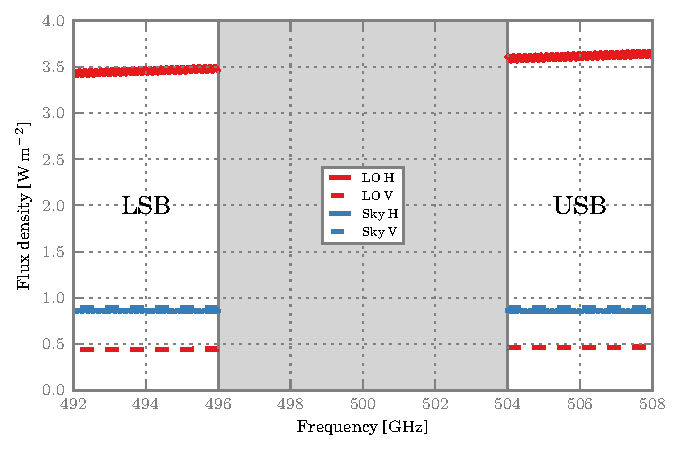
\includegraphics{thin_film_beam_splitter_detailed}
    \caption{Thin film beam splitter, detailed}
    \label{fig:thin_film_beam_splitter_detailed}
\end{figure}
In the lower and upper side bands, the mixer receives power from two sources: the astronomical signal from the sky and the noise of the local oscillator.
In the case of HIFI, the local oscillator noise is typically two orders of magnitude stronger than the astronomical signal.
We arbitrarily set the power density from the sky at \SI{1}{\watt\per\meter\squared} and that of the local oscillator to \SI{100}{\watt\per\meter\squared}.
Since these two sources are not phase locked, we solve the system for each of them independantly.
The result is given on \cref{fig:thin_film_beam_splitter_detailed}.

We notice that the power of both the local oscillator signal and the sky signal have the same order of magnitude when hitting the mixer.
This is due to the fact that the thin film is mostly transparent, hardly reflective.
Because the sky is seen in transmission, its power is still very close to its emitted value of \SI{1}{\watt\per\meter\squared}, we couple most of the sky.
And because the local oscillator is seen in reflection, we couple only a small fraction of it (\SI{0.5}{\percent} or \SI{3.5}{\percent} depending on the polarization).
This increases the signal-to-noise ratio to an acceptable level.

The figure also illustrates that this beam splitter transmits V more than it transmits H.
As a result, V shows more sky power and less LO power.
It is in the interest of the astronomer to reject the horizontal polarization.
This can be done with a wire-grid polarizer or by using rectangular horns.

When examined closely, the H curves show some fast oscillations.
The V curves are also affected, as the next figure will show.
These oscillations are due to the cavity formed by the mixer and the local oscillator.
That cavity consists of $d=\SI{1}{\meter}$ or vacuum, which results in a period of $c_0 / 2d \approx \SI{150}{MHz}$.

The red curves show a slope.
The higher the frequency, the more LO power the mixer sees.
This slope is actually a portion of a very slow standing wave pattern.
It corresponds to the cavity formed by the two interfaces of the thin film itself.
With a speed of light of $c_0 / 1.83$ and a thickness of \SI{10}{\micro\meter}, we expect a standing wave pattern with a period of about \SI{8}{\tera\hertz}.
Calculating the real period involves knowing the pathlength of the beam inside the film, which requires some trigonometry, but the order remains at several terahertz.

In a real system, we would not have access to all the details of \cref{fig:thin_film_beam_splitter_detailed}.
Indeed, for a given frequency, we receive the sum of the LO and sky power without being able to tell them apart.
Furthermore, mixers fold spectra, which adds the lower and upper side bands together.
Finally, the polarizations become undistinguishable.
In \cref{fig:thin_film_beam_splitter_folded}, we have summed the two sources and folded the spectra; however we kept the polarization intact.
These summations were done in power and not in field, because the LSB, USB, LO and sky power are not phase locked to each other: each signal is coherent with itself only, not with the others.

\begin{figure}[hbtp]
    \centering
    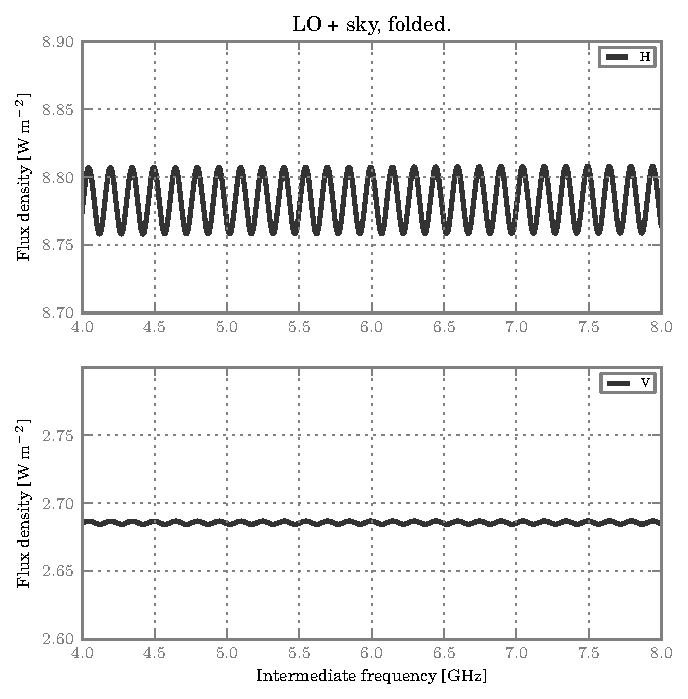
\includegraphics{thin_film_beam_splitter_folded}
    \caption{Thin film beam splitter, folded}
    \label{fig:thin_film_beam_splitter_folded}
\end{figure}

The slope due to the cavity inside the thin film seems to have disappeared.
This is expected: the lower sideband is flipped before being added to the upper sideband.
Therefore, when the slope goes up for one, it goes down for the other,
and they compensate quite well.
Some other values for the LO frequency or film thickness can allow the thin film cavity to leave a more obvious signature on the folded spectrum.

This figure reveals that the V polarization is also affected by standing wave, as we mentionned earlier.
It is much weaker in V than in H because the thin film is more transparent for V.
This means that the V-polarized light is more likely to exit the cavity either toward the sky or toward the open port on the right, both perfect aborbers.
This standing wave pattern has a period of \SI{150}{\mega\hertz}, which is expected of the LO--mixer cavity.

\subsubsection{Sideband ratio}
Standing waves change the coupling of the mixer to the signal.
This coupling is a priori different in the lower and upper sideband.
Therefore, each channel of a folded spectrum is a priori imbalanced, giving more weight to either sideband.

In the HIFI consortium, we agreed on the following definition~\eqref{eq:sideband_ratio} of the sideband ratio as a metric for the imbalance between the two sidebands.
A perfectly balanced system has a sideband ratio of 0.5.
If the sideband ratio is greater than 0.5, then the channel is USB-dominated.
If it is lower than 0.5, the channel is LSB-dominated.
\begin{equation}
    \text{sideband ratio} =
    \frac{
        \text{USB power coupling}
    }{
        \text{LSB power coupling} + \text{USB power coupling}
    }
    \label{eq:sideband_ratio}
\end{equation}

\begin{figure}[hbtp]
    \centering
    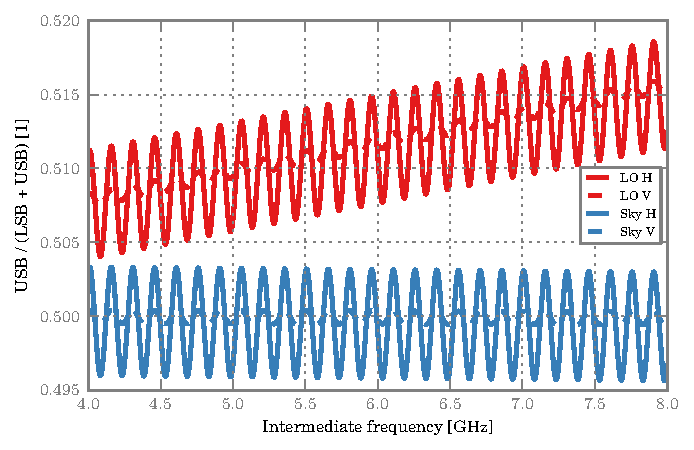
\includegraphics{thin_film_beam_splitter_sbr}
    \caption{Thin film beam splitter, sideband ratio}
    \label{fig:thin_film_beam_splitter_sbr}
\end{figure}
\Cref{fig:thin_film_beam_splitter_sbr} shows the sideband ratio for the LO and the sky for both polarizations.
The slope comes from very slow modulation due to the cavity inside the thin film.
Note that it is clearly visible here, even on the sky, while it was hardly noticeable on the folded spectrum of \cref{fig:thin_film_beam_splitter_folded}.
A flat continuum does not guarantee a flat sideband ratio.

With this system, the standard deviation of the sideband ratio for is \SI{2.6}{\percent} for H and \SI{0.3}{\percent} for V.
This is the error that we can expect when measuring a thin emission line on a perfectly flat continuum after an infinitely long integration time: the line can fall anywhere between a peak and a crest of this standing wave pattern.

\subsubsection{The many LO--mixer cavities}

\Cref{fig:thin_film_beam_splitter_folded_fft} shows
the fast Fourier Transform of \cref{fig:thin_film_beam_splitter_folded} (using a Hanning window).
It peaks at the expected~\SI{150}{\mega\hertz} and shows a very weak harmonic at~\SI{75}{\mega\hertz}.
The harmonics are very weak because the cavity is of very low quality: the film is very transparent and the light leaves the cavity quickly.

\begin{figure}[hbtp]
    \centering
    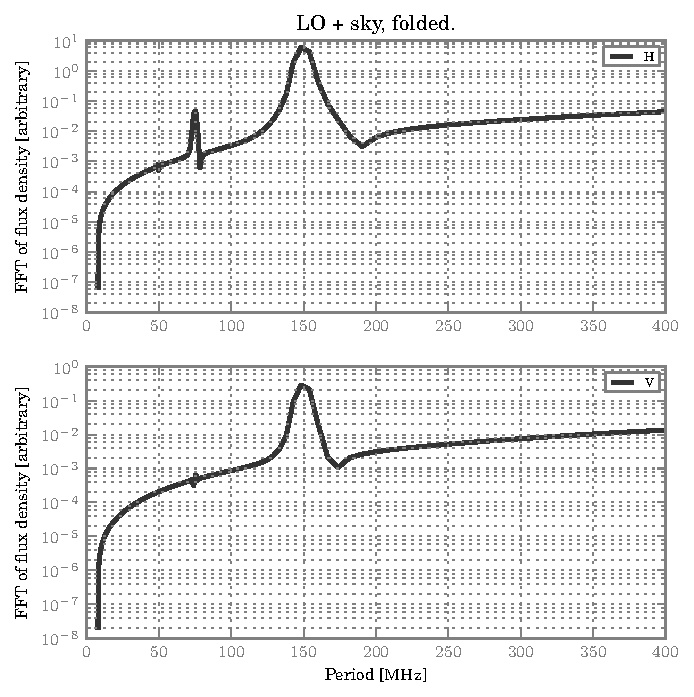
\includegraphics{thin_film_beam_splitter_folded_fft}
    \caption{Thin film beam splitter, folded, fft}
    \label{fig:thin_film_beam_splitter_folded_fft}
\end{figure}

The astute reader may be wondering why we are observing only two cavities (LO--mixer and inside thin film) instead of an infinity.
Indeed, there is no such thing as \textit{the} LO--mixer cavity, there are an infinity of them.
The shortest one is the one corresponding to a single reflection on the near side of the thin film.
Then, another possible path involves entering the thin film, being reflected by the far side, traversing the film again, and being transmitted toward the detector.
A third path involves two round-trips inside the film, and a fourth path involves three round-trips, etc.
Why don't these many cavities show up as as many peaks on the FFT?
The answer is simple: our FFT does not have enough resolution.

Our bandpass $B$ of \SI{4}{\giga\hertz} does not allow to resolve a variation of \SI{10}{\micro\meter} in a cavity.
$B = c / 2d$ with $d=\SI{10}{\micro\meter}$ and $c=c_0$ yields $B \approx \SI{15}{\tera\hertz}$, which is way beyond our \SI{4}{\giga\hertz}.
If we reverse the calculation, $d=c/2B$ for $B=\SI{4}{\giga\hertz}$ gives $d \approx \SI{37}{mm}$: our FFT can distinguish cavities that differ by more than \SI{4}{\centi\meter}.
This limitation affects only the FFT as a tool used for visualizing our data; our model has no such limitation.

\begin{figure}[hbtp]
    \centering
    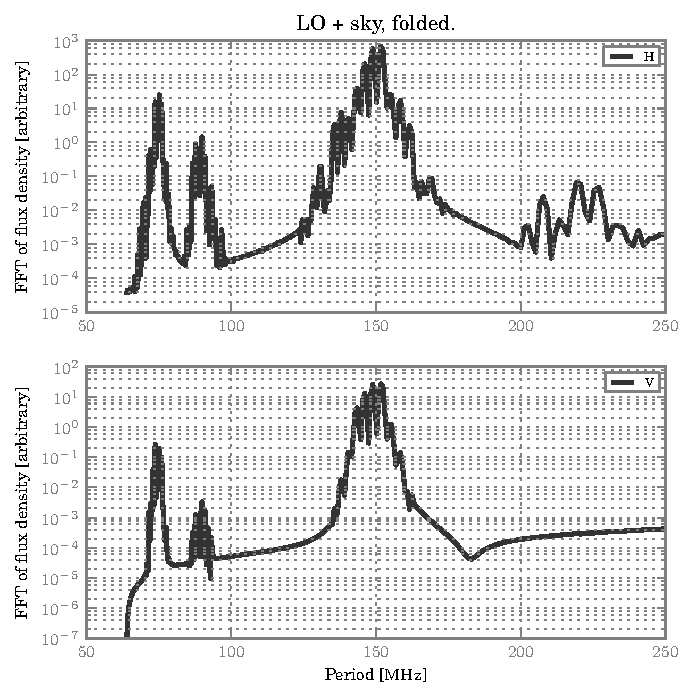
\includegraphics{thin_film_beam_splitter_folded_fft_hr}
    \caption{Thin film beam splitter, folded, fft, high resolution}
    \label{fig:thin_film_beam_splitter_folded_fft_hr}
\end{figure}
\Cref{fig:thin_film_beam_splitter_folded_fft_hr} shows the FFT of the same system for a bandwidth of~\SI{32}{\giga\hertz}, a film thickness of~\SI{1}{\centi\meter}, and no imaginary part in the refractive index of the mylar (otherwise the absorption would hide the result).
Once the system is modified to meet the expectations of the FFT, then the FFT does show the expected many peaks around~\SI{150}{\mega\hertz}, which prove that our model takes into account the infinity of LO--mixer cavities.
